%% 美赛模板:正文部分

\documentclass[12pt]{article}  % 官方要求字号不小于 12 号,此处选择 12 号字体

% 本模板不需要填写年份,以当前电脑时间自动生成
% 请在以下的方括号中填写队伍控制号
\usepackage[2510086]{easymcm}  % 载入 EasyMCM 模板文件
\problem{C}  % 请在此处填写题号
% \usepackage{mathptmx}  % 这是 Times 字体,中规中矩 
\usepackage{mathpazo}  % 这是 COMAP 官方杂志采用的更好看的 Palatino 字体,可替代以上的 mathptmx 宏包
\usepackage{longtable}
\usepackage{float}
\usepackage{booktabs}
\usepackage{multirow}
\usepackage{graphicx}
\usepackage{adjustbox}
\usepackage{caption}
\usepackage{listings}
\lstset{basicstyle=\footnotesize, % Adjust this value as needed
        breaklines=true, % Allows code to break across lines
        frame=single}   % Optional: Adds a frame around the code block
\title{A Dive Into the Prediction of Olympic Medal Counts}  % 标题

\renewcommand{\contest}{MCM}

% 文档开始
\begin{document}

% 此处填写摘要内容
\begin{abstract}
This study investigates Olympic Medal Count Prediction through \textbf{Machine Learning }and \textbf{Statistical Modeling Techniques}. By analyzing historical data, we tackle five key tasks to uncover trends and develop predictive models that offer valuable insights into medal outcomes and strategies for improving performance.

In Task 1, we implement a sliding window approach to capture temporal dependencies in features such as athletes, events, sports, and medal counts. The \textbf{RidgeCV Regression Model}, which handles multicollinearity through L2 regularization, outperforms models like Linear Regression, Lasso, ElasticNet, and SVR with a variance score of \textbf{0.95} and \textbf{RMSE} of \textbf{4.71}. \textbf{Bootstrapping} is used to estimate confidence intervals for robust medal predictions, with a table detailing the top 20 countries’ predictions. The USA, China, and Great Britain are expected to dominate, while Germany, Czech Republic, and Poland will see improvements, and countries like France, South Korea, and Australia may decline.

In Task 2, we aim to predict the number and probability of countries winning their first medal in the 2028 Olympics. We develop the \textbf{Bayesian-Optimized XGBoost Medal Predictor (BO-XGMP)}, optimizing XGBoost’s hyperparameters using Bayesian methods. The model achieves an accuracy of \textbf{0.90} and an AUC of \textbf{0.86} on the test set. Finally, we use a \textbf{Linear Regression Model} to fit the data for 2028, predicting that \textbf{2 countries} have the highest probability (\textbf{0.29}) of winning their first Olympic medal.

In Task 3, we first investigate the relationship between the number and categories of events and their impact on medal counts. By analyzing the number of athletes participating in various event types and creating a correlation matrix, the research aims to uncover patterns that influence performance outcomes. Secondly, we develop the \textbf{EWM-TOPSIS Model} to assess the most important events for various countries, using the \textbf{Entropy Weight Method} for weight assignment and TOPSIS for the solution. Using China as an example, we input the data into the model, and the model highlights Table Tennis as the most significant event. Thirdly, we quantify the performance of the host country and all athletes in newly added events, applying the \textbf{Mann-Whitney U test}. The \textbf{p-value of 0.596} indicates no significant impact of host country-chosen events on results.

In Task 4, we analyze the "great coach" effect, highlighting Béla Károlyi’s impact on the USA gymnastics team\textbf{}’s 2016 Olympic performance, where actual medal counts exceed predictions. We estimate that exceptional coaching could increase medal counts by around \textbf{10\%}, as per the Fibonacci Weighted Point System. The analysis suggests \textbf{India} (athletics), \textbf{Brazil} (swimming), and \textbf{South Africa} (boxing) could benefit from such coaching expertise to improve in these sports. 

In Task 5, we identify a pattern linking countries' first medals to specific sports, enabling us to recommend key sports for countries yet to win a medal. We develop a recommendation equation, optimized using \textbf{BO-XGMP} predictions and sports data, and provide sport recommendations for \textbf{MYA}, \textbf{MLT}, \textbf{MLI}, and \textbf{GBS}.



    % 美赛论文中无需注明关键字。若您一定要使用,
    % 请将以下两行的注释号 '%' 去除,以使其生效
\vspace{5pt}
\textbf{Keywords}: RidgeCV, BO-XGMP, EWM-TOPSIS, Mann-Whitney U test.

\end{abstract}

\maketitle  % 生成 Summary Sheet
\tableofcontents  % 生成目录


% 正文开始
\section{Introduction}
\subsection{Problem Background and Literature Review}
During the most recent 2024 Paris Summer Olympics, aside from watching the competitions, spectators were also very interested in the medal tally of various countries. The nations at the top of the rankings always attract a lot of attention, and everyone hopes their own country can be among the leaders.

Over the past several decades of Olympic Games, many "sporting powerhouses" have emerged, but there are also numerous countries still striving to win their first Olympic medal in history. How will these medal-winning countries perform in the next Olympics? And do those countries without any medals have a chance to win one? These are all questions that people are concerned about.

Predictions of the final medal count are common, but they are typically not based on historical medal totals. Instead, they are often made just before the opening of the upcoming Olympics, when the athletes scheduled to compete are known\cite{1}. However, when the information about the planned participants has not been disclosed, as is the case now with the 2028 Los Angeles Olympics where the competing athletes have yet to be announced, can we still predict the medal outcomes for various countries? This is the question that concerns us.

Past research has focused on exploring the application of machine learning techniques to predict medal outcomes and analyze medal distribution patterns for the 2024 Summer Olympics\cite{2}. Leveraging a wide range of variables at both athlete and country levels, as well as event-specific metrics, various statistical models are employed to forecast medal counts and identify factors linked to Olympic success. However, such research methods cannot proceed without information on the participants of the next Olympic Games. This necessitates that we seek solutions within the limited dataset available to us.

\subsection{Restatement of the Problem}

\begin{enumerate}[\textbullet]
    \item \textbf{Task 1:} Project the 2028 LA Olympics medal table using your model, including prediction intervals. Identify countries likely to improve or decline compared to 2024.
    \item \textbf{Task 2:} Predict how many countries will win their first medal in 2028 and estimate the odds of this outcome.
    \item \textbf{Task 3:} Analyze how event types and numbers affect medal counts. Identify key sports for different countries and the impact of host-selected events.
    \item \textbf{Task 4:} Investigate the "great coach" effect on medal counts. Suggest three countries and sports where hiring such a coach could have significant impact.
    \item \textbf{Task 5:} Share original insights from your model to guide national Olympic committees' decisions.
\end{enumerate}

\subsection{Our work}
For ease of description and visualization, we have drawn a flow chart (Figure 1) to represent our work.
\begin{figure}[h]
    \centering
    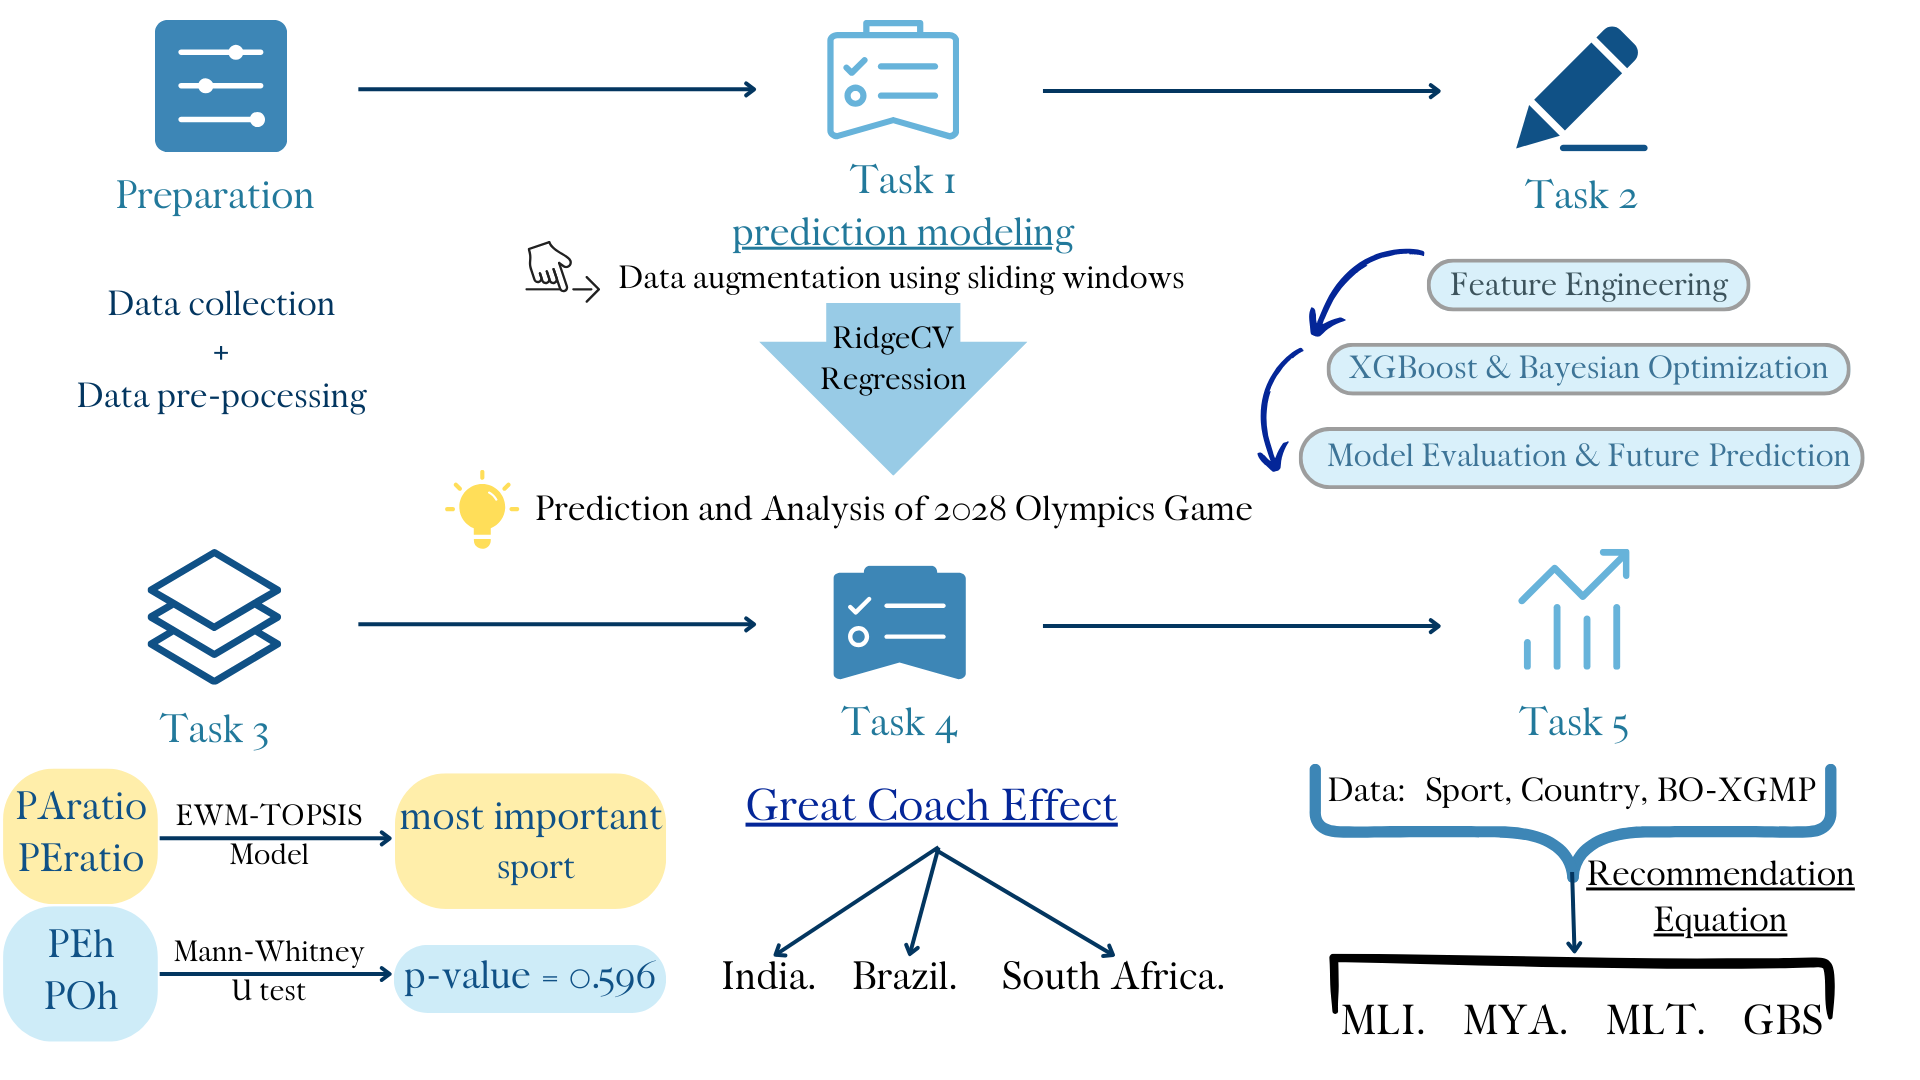
\includegraphics[width=0.75\linewidth]{#67B3DA.png}
    \caption{Our Work}
    \label{fig:enter-label}
\end{figure}


\section{Assumptions}
\begin{itemize}
\item The medal count of a country is directly influenced by the total number of athletes it fields, assuming that athletes possess similar levels of ability. A larger athlete pool increases the likelihood of winning medals.
\item The format, number of events, and competition conditions (e.g., scoring systems, rules) remain consistent across Olympic Games.
\item External factors, such as geopolitical tensions, doping scandals, or unexpected changes in sponsorship, do not drastically alter a country’s medal performance from one Olympic Games to the next.
\end{itemize}
\section{Notations}
The primary notations used in this paper are listed in Table \ref{tb:notation}.

% 三线表示例
\begin{table}[!htbp]
\begin{center}
\caption{Notations}
\begin{tabular}{cl}
	\toprule
	\multicolumn{1}{m{3cm}}{\centering Symbol}
	&\multicolumn{1}{m{8cm}}{\centering Definition}\\
	\midrule
	$X$&Features\\
	$y$&Target\\
        $w$&Weight\\
	$\alpha$ &Ridge Parameter\\
        $\beta$ &vector of regression coefficient\\
        $l$&Loss\\
        $PE$&Performance Score\\
        $P$&Number of Participants\\
        $N$&Total Number of Countries\\
        
        
	\bottomrule
\end{tabular}\label{tb:notation}
\end{center}
\end{table}

\section{Data Pre-processing}
Upon organizing the data, it becomes evident that there are inconsistencies between the format of the provided data and the required format specified in the question. To address this, it is crucial to preprocess the data accordingly. The first step involves standardizing the data headers to ensure consistency, followed by the abbreviation of the indicators to enhance clarity and streamline the subsequent listing. Detailed information regarding the specific formatting and abbreviations used can be seen as follow.
\begin{longtable}{|c|l|}
\hline
\textbf{Abbreviation} & \textbf{Description} \\
\hline
\endfirsthead
\hline
\textbf{Abbreviation} & \textbf{Description} \\
\hline
\endhead
\hline
\endfoot

Year & Olympic Games year \\
NOC & Participating country \\
Host & Host country or not (1: yes, 0: no) \\
Athletes & Number of athletes \\
Females & Number of female athletes \\
Sports & Number of unique sports \\
Events & Number of unique events \\
\end{longtable}

The provided data contains several inconsistencies. For instance, countries are described in various formats, and we have standardized these descriptions using the NOC abbreviation. Similarly, different representations of the same events exist, and we have unified these as well. Additionally, when counting the total number of medals earned by athletes from a given country, we found discrepancies between the numbers derived from the "summerOly athletes.csv" file and those from the "summerOly medal counts.csv" file. To ensure accuracy, we will rely on the medal counts from the "summerOly medal counts.csv" for the final medal tally.
\section{Task 1: Estimating Future Medal Counts for Each Country}

\subsection{Data augmentation using sliding windows}
The organized features alone are insufficient for accurately predicting Olympic performance. Given that we are working with time series data, it is crucial to incorporate the historical context of previous performances. To achieve this, we apply the concept of a sliding window. This technique helps our model capture temporal dependencies by accounting for the uncertainty inherent in the progression of the games, while evaluating a country's performance over a recent sequence of events. Specifically, for features such as "Athletes," "Events," "Sports," "Females," "Real Gold", "Real Silver" and "Real Bronze" we use the sliding window approach to augment the dataset. In this case, we implement 9 distinct sliding windows to enrich the model's ability to learn from past data and improve its predictive power.
\begin{figure}[H]
    \centering
    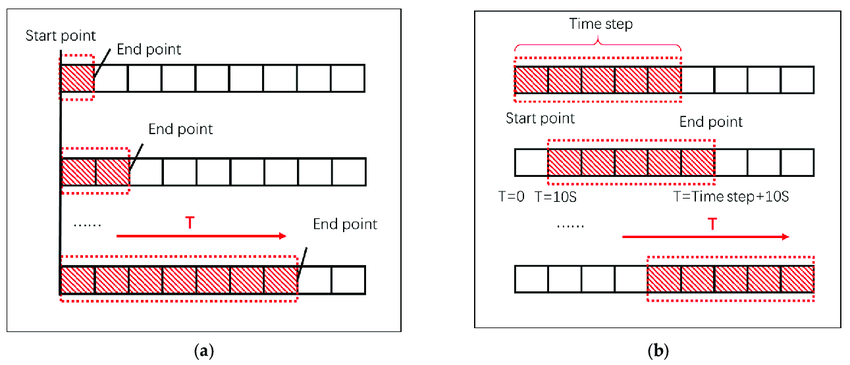
\includegraphics[width=0.5\linewidth]{sliding window.png}
    \caption{Sliding windows}
    \label{fig:enter-label}
\end{figure}

\subsection{RidgeCV Regression}
Ridge regression stabilizes coefficients in multiple regression models with highly correlated independent variables by adding a ridge parameter (bias) to the correlation matrix. RidgeCV extends this by using cross-validation to automatically tune the ridge parameter (alpha). Unlike Ridge, Ordinary Least Squares (OLS) minimizes the difference between predicted and actual values without regularization. The objective of OLS is to minimize the sum of squared errors:

\begin{equation}
    \hat{\beta} = \arg \min_{\beta} \| y - X \beta \|^2 \tag{1}
\end{equation}


where \( X \) is the matrix of independent variables, \( y \) is the vector of the dependent variable, and \( \beta \) is the vector of regression coefficients. The solution to this optimization problem is:

\begin{equation}
    \hat{\beta} = (X^T X)^{-1} X^T y \tag{2}
\end{equation}


However, a problem arises when the independent variables are highly correlated (for example, when house size and number of rooms are strongly related). In this case, the matrix \( X^T X \) may become nearly singular, with its determinant close to zero, which causes \( (X^T X)^{-1} \) to become unstable. This leads to highly volatile estimates of \( \beta \), resulting in high variance and poor prediction performance.
Ridge Regression addresses the issue of multicollinearity by adding a regularization term \( \alpha \| \beta \|^2 \) to the OLS objective function. The modified objective function becomes:

\begin{equation}
    \hat{\beta} = \arg \min_{\beta} \left( \| y - X \beta \|^2 + \alpha \| \beta \|^2 \right) \tag{3}
\end{equation}



where \( \lambda \) is the ridge parameter, and \( I \) is the identity matrix. The solution to this objective function is:

\begin{equation}
    \hat{\beta} = (X^T X + \alpha I)^{-1} X^T y \tag{4}
\end{equation}


Key points to consider:

\begin{itemize}
    \item The regularization term \( \alpha \| \beta \|^2 \) helps prevent large regression coefficients, thereby reducing the model's complexity.
    \item As \( \lambda \) increases, the regression coefficients shrink, lowering the model's variance but introducing some bias.
    \item By selecting an appropriate value for \( \alpha \), Ridge Regression can find a balance between bias and variance, which improves the model's predictive performance.
\end{itemize}

Ridge regression, using L2 regularization, reduces dimensionality and overfitting by controlling model parameters, making it effective for correlated datasets and outliers. RidgeCV optimizes the regularization parameter \( \alpha \) via cross-validation, improving model fit. Unlike Lasso, which can eliminate variables with L1 regularization, Ridge retains all predictors, ensuring a stable, interpretable model, particularly when all features are significant.


\begin{figure}[H]
    \centering
    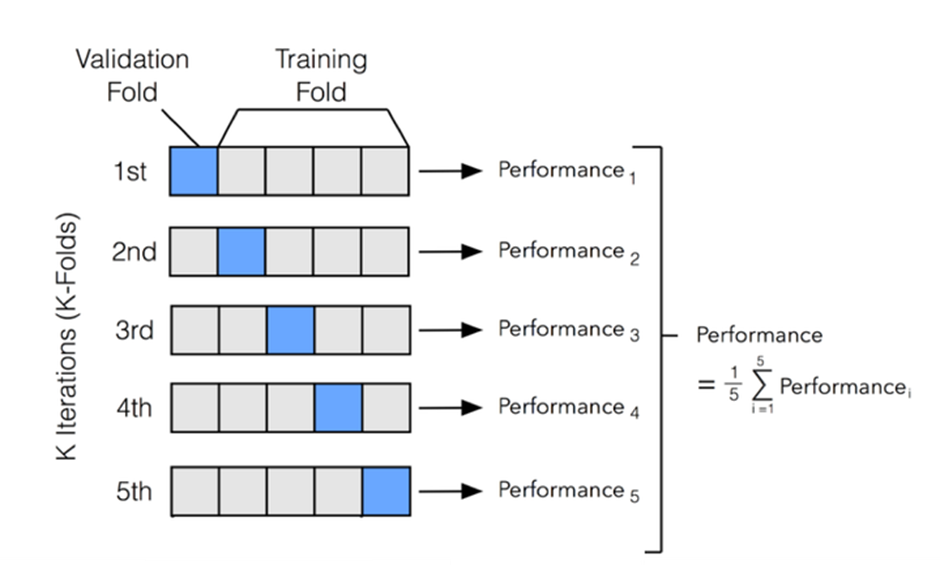
\includegraphics[width=0.5\linewidth]{crossValidation.png}
    \caption{Cross Validation illustration}
    \label{fig:enter-label}
\end{figure}
\subsection{Model Evaluation of RidgeCV algorithm}
We split the dataset into training and testing sets, using an 80:20 ratio. Various machine learning algorithms were applied to fit the data, including Linear Regression, Lasso Regression, ElasticNet Regression, and Support Vector Regression (SVR). The performance of these models was evaluated using the variance score and root mean squared error (MSE) on test set. Our results showed that RidgeCV consistently outperformed all other models across these metrics.

\begin{table}[H]
\centering
\begin{tabular}{lcc}
\toprule
\textbf{Models} & \textbf{Variance Score} & \textbf{RMSE} \\
\midrule
RidgeCV         & 0.95                    & 4.71         \\
Linear Regression & 0.91                  & 6.11         \\
Lasso           & 0.88                    & 7.05         \\
ElasticNet      & 0.88                    & 7.05         \\
SVR             & 0.31                    & 16.97        \\
Neural Network  & 0.21                    & 18.91        \\
\bottomrule
\end{tabular}
\caption{Performance of different models evaluated by Variance Score and RMSE.}
\label{tab:model_performance}
\end{table}
\subsection{Applying bootstrapping to estimate confidence intervals}
To estimate the confidence interval for the predicted medal numbers, we employ the bootstrapping method.The bootstrapping method is a statistical technique used to estimate the distribution of a sample statistic by resampling with replacement from the observed data. It allows for the estimation of properties like confidence intervals or standard errors without making strong assumptions about the underlying data distribution.

The confidence interval (CI) for a statistic like the mean using bootstrapping can be expressed as:

\begin{equation}
    \text{CI} = \left[ \text{percentile}_{\frac{\alpha}{2}}, \text{percentile}_{1-\frac{\alpha}{2}} \right] \tag{5}
\end{equation}


Where:

\begin{itemize}
    \item \( \alpha \) is the desired significance level (e.g., 0.05 for a 95\% confidence interval).
    \item The percentiles correspond to the lower and upper bounds of the confidence interval, based on the bootstrap distribution.
\end{itemize}
\begin{figure}[H]
    \centering
    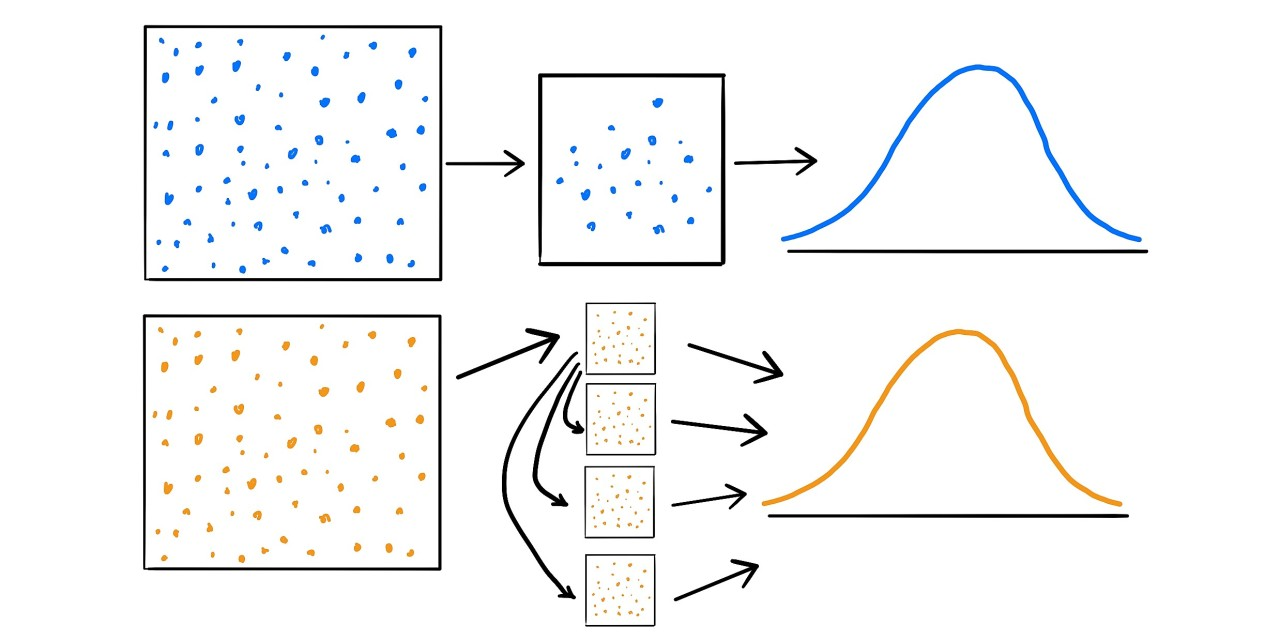
\includegraphics[width=0.5\linewidth]{Bootstrapping.png}
    \caption{Bootstrapping Illurstration}
    \label{fig:enter-label}
\end{figure}
\subsection{The prediction and analysis of 2028 Olympics Game}
By combining RidgeCV and bootstrapping, we successfully predicted the medal counts for the 2028 Olympic Games. Below are the results for the top 20 countries, sorted by their predicted total medal counts.
\begin{table}[H]
\centering
\adjustbox{max width=\textwidth, valign=c}{ % Adjust the table to fit the width
\begin{tabular}{|c|c|c|c|c|c|c|c|c|c|c|c|c|}
\hline
\textbf{NOC} & \textbf{Golds} & \textbf{Gold\_low} & \textbf{Gold\_up} & \textbf{Silvers} & \textbf{Silver\_low} & \textbf{Silver\_up} & \textbf{Bronzes} & \textbf{Bronze\_low} & \textbf{Bronze\_up} & \textbf{Medals} & \textbf{Medals\_low} & \textbf{Medals\_up} \\
\hline
 USA  & 49 & 38 & 59  & 37 & 27 & 45  & 35 & 25 & 40 & 121 & 90 & 144 \\
 CHN  & 35 & 21 & 43  & 25 & 10 & 33  & 24 & 12 & 33 & 84  & 43 & 109 \\
 GBR  & 21 & 14 & 30  & 18 & 8  & 26  & 19 & 11 & 26 & 58  & 33 & 82 \\
 GER  & 13 & 2  & 21  & 14 & 8  & 23  & 21 & 15 & 28 & 48  & 25 & 72 \\
 FRA  & 15 & 11 & 19  & 14 & 9  & 18  & 18 & 13 & 23 & 47  & 33 & 60 \\
 AUS  & 14 & 7  & 20  & 12 & 6  & 18  & 18 & 13 & 22 & 44  & 26 & 60 \\
 JPN  & 15 & 9  & 20  & 12 & 6  & 16  & 16 & 12 & 20 & 43  & 27 & 56 \\
 ITA  & 12 & 10 & 16  & 12 & 10 & 15  & 14 & 12 & 17 & 38  & 32 & 48 \\
 CAN  & 8  & 4  & 13  & 10 & 6  & 14  & 12 & 8  & 15 & 30  & 18 & 42 \\
 NED  & 9  & 6  & 13  & 9  & 7  & 14  & 11 & 7  & 14 & 29  & 20 & 41 \\
 KOR  & 9  & 0  & 14  & 7  & 0  & 12  & 6  & 0  & 12 & 22  & 0  & 36 \\
 ESP  & 4  & 0  & 8   & 8  & 4  & 12  & 9  & 6  & 15 & 21  & 10 & 35 \\
 HUN  & 7  & 5  & 11  & 6  & 4  & 9   & 7  & 4  & 10 & 20  & 13 & 30 \\
 BRA  & 4  & 0  & 8   & 6  & 2  & 10  & 8  & 4  & 11 & 18  & 6  & 29 \\
 POL  & 5  & 2  & 8   & 5  & 2  & 8   & 7  & 4  & 10 & 17  & 8  & 26 \\
 NZL  & 6  & 4  & 9   & 5  & 2  & 7   & 6  & 3  & 8  & 17  & 9  & 24 \\
 UKR  & 3  & 0  & 9   & 3  & 0  & 7   & 8  & 1  & 13 & 14  & 1  & 29 \\
 SWE  & 3  & 1  & 6   & 5  & 1  & 7   & 5  & 3  & 8  & 13  & 5  & 21 \\
 CUB  & 4  & 0  & 7   & 3  & 2  & 6   & 5  & 2  & 8  & 12  & 2  & 22 \\
\hline
\end{tabular}
}
\caption{Predicted Medal Counts for the 2028 Olympic Games: Top 20 Countries}
\label{tab:medal_counts}
\end{table}
We also identified the top 10 countries expected to show improved performance in the 2028 Olympics compared to the 2024 Games, based on predicted medal counts. Conversely, we highlighted 10 countries projected to experience a decline in performance, with fewer medals anticipated in 2028 compared to 2024.
\begin{table}[h!]
\centering
\begin{minipage}{0.45\textwidth}
    \centering
    \resizebox{\textwidth}{!}{ % Adjust the table to fit the text width
    \begin{tabular}{|c|c|c|c|c|}
    \hline
    \textbf{NOC} & \textbf{Gold\_char} & \textbf{Silver\_char} & \textbf{Bronze\_char} & \textbf{Medal\_char} \\
    \hline
    GER & 1  & 1  & 13 & 15 \\
    CZE & 1  & 3  & 3  & 7  \\
    POL & 4  & 1  & 2  & 7  \\
    KAZ & 2  & 0  & 2  & 4  \\
    CAN & -1 & 3  & 1  & 3  \\
    DEN & 1  & 2  & 0  & 3  \\
    ROU & 0  & 0  & 3  & 3  \\
    CUB & 2  & 2  & -1 & 3  \\
    ESP & -1 & 4  & 0  & 3  \\
    DMA & 1  & 1  & 1  & 3  \\
    \hline
    \end{tabular}
    }
    \caption{Top 10 Countries with Better Performance in the 2028 Olympics}
    \label{tab:better_performance}
\end{minipage}%
\hspace{0.5cm} % Adjust the space between the tables
\begin{minipage}{0.45\textwidth}
    \centering
    \resizebox{\textwidth}{!}{ % Adjust the table to fit the text width
    \begin{tabular}{|c|c|c|c|c|}
    \hline
    \textbf{NOC} & \textbf{Gold\_char} & \textbf{Silver\_char} & \textbf{Bronze\_char} & \textbf{Medal\_char} \\
    \hline
    ARM & 0  & -3 & -1 & -4 \\
    BRN & -2 & -1 & -1 & -4 \\
    NED & -6 & 2  & -1 & -5 \\
    KGZ & 0  & -2 & -3 & -5 \\
    USA & 9  & -7 & -7 & -5 \\
    GBR & 7  & -4 & -10 & -7 \\
    CHN & -5 & -2 & 0  & -7 \\
    AUS & -4 & -7 & 2  & -9 \\
    KOR & -4 & -2 & -4 & -10 \\
    FRA & -1 & -12 & -4 & -17 \\
    \hline
    \end{tabular}
    }
    \caption{Top 10 Countries with Worse Performance in the 2028 Olympics}
    \label{tab:worse_performance}
\end{minipage}
\end{table}

\section{Task 2: Predicting the Probability of Countries Winning Their First Medal}


In this section, we identify patterns in countries transitioning from no medals to their first Olympic medal, predicting how many countries will win their first medal in the upcoming Games and their probabilities. We preprocessed the data, selected three key features, and trained an XGBoost model optimized with Bayesian tuning. Finally, we apply the model to the 2028 Olympic data to generate predictions.

\subsection{Feature Engineering}

This study focuses on identifying patterns in countries’ progression from not winning medals to winning their first. We pre-process athlete data by retaining records from countries with no medals or those winning their first medal in a given Olympic Games, while removing anomalous data, such as Russia’s exceptional performance due to historical factors, and excluding data from the refugee team, which started competing in 2016.

Next, we select $N_i$, $P_i$, and $E_i$ as the input features. Here, $N_i$ denotes the $i^{th}$ country's participation number, $P_i$ represents the number of athletes sent, and $E_i$ is the number of events entered. The output feature, $F_i$, indicates whether the country won a medal (1) or not (0). Therefore, the input vector for each country is represented as:
\begin{equation}
    \mathbf{x}_i = (N_i, P_i, E_i) \tag{6}
\end{equation}

and the corresponding output is:

\begin{equation}
    y_i = F_i \tag{7}
\end{equation}


In total, we process and organize \textbf{1,244} vectors representing the various features of each country's participation and medal achievement across different Olympic Games.

\subsection{Bayesian-Optimized XGBoost Medal Predictor (BO-XGMP)}

Chen et al. developed the \textbf{eXtreme Gradient Boosting (XGBoost)} algorithm, which leverages an optimized distributed gradient boosting technique to quickly train datasets while maintaining efficient resource utilization and high accuracy\cite{4}. In this problem, we aim to predict how many countries will win their first medal at the next Olympic Games, and estimate the probability of this occurrence.
The dataset consists of only 1244 samples, with a significant imbalance between the number of countries that have won medals and those that have not, making the task inherently imbalanced. XGBoost has demonstrated excellent performance in addressing imbalanced and small-sample binary classification problems\cite{5}\cite{6}. By using the binary:logistic loss function, it directly outputs probabilities, which is ideal for this task. Additionally, we employ Bayesian optimization to fine-tune the hyper-parameters of XGBoost to further enhance the model's performance\cite{7}.

\begin{enumerate}[\textbullet]
    \item \textbf{Model Construction: XGBoost and Bayesian Optimization}

\textbf{A. XGBoost}

The XGBoost objective function consists of two components: the loss function and the regularization term, both of which work together to optimize the model. The objective function is expressed as:
\[
L(\theta) = \sum_{i=1}^{n} \ell(y_i, \hat{y}_i) + \Omega(\theta) \tag{8}
\]
where \(\ell(y_i, \hat{y}_i)\) represents the loss function, which measures the error for the \(i^{th}\) sample, and \(\Omega(\theta)\) is the regularization term, which controls the model's complexity to prevent overfitting.

For binary classification, the loss function used is log-loss:
\[
\ell(y_i, \hat{y}_i) = - y_i \log(\hat{y}_i) - (1 - y_i) \log(1 - \hat{y}_i) \tag{9}
\]
where \(y_i\) is the actual label (0 or 1) for the \(i^{th}\) sample, and \(\hat{y}_i\) is the predicted probability that the sample belongs to class 1. The loss function minimizes the difference between the predicted probabilities and the actual labels.

The regularization term is defined as:
\[
\Omega(\theta) = \gamma T + \frac{1}{2} \lambda \sum_{j=1}^{k} \theta_j^2 \tag{10}
\]
where \(T\) is the number of trees, \(\gamma\) controls the complexity of the trees, and \(\lambda\) controls the size of the leaf weights. This regularization term penalizes overly complex models, reducing the risk of overfitting and ensuring better generalization.

\textbf{B. Bayesian Optimization}

\textbf{Bayesian Optimization (BO)} uses historical evaluation results to select optimal hyperparameter combinations based on their distribution\cite{8}. It uses \textbf{Gaussian Processes (GP)} to model the relationship between the model error $\vartheta_Z$ and its parameters $p_Z$. A set of $Z$ points generates a multivariate Gaussian distribution in $\mathbb{R}^Z$. With prior Gaussian processes derived from previous experiments, a posterior function $\alpha(p)$ is constructed, where the acquisition function (AC) depends on the predictive mean function $\hat{\mu}(p)$ and the predictive variance function $\sigma^2(p)$.

To determine the next sampling point, the Bayesian optimization model maximizes $p_{\text{next}} = \arg \max_p \alpha(p)$, balancing the exploration of areas with high variance and the exploitation of regions with low mean. The \textbf{Gaussian Process Upper Confidence Bound (GP-UCB)} acquisition function is used to control the exploration-exploitation trade-off, with the parameter $\kappa$ adjusting the balance:
\begin{equation}
    \alpha_{UCB} = \varpi(\mathbf{p}) - \kappa \sigma(\mathbf{p}) \tag{11}
\end{equation}

This method demonstrates strong performance in hyper-parameter tuning by efficiently navigating the search space.

\item \textbf{Model Solution}

\textbf{(1) Model Training:} Since countries' first medal achievements vary significantly—for instance, San Marino (SMR) won 2 silvers and 2 bronzes in their first appearance—while many countries win only a bronze, we aim to differentiate these cases. To address this, we apply the Fibonacci Weighted Point System proposed by Sergeyev to quantify performance\cite{3}.
    
    The performance score for a country's team in the $i^{th}$ Olympic Games is calculated as follows:
    \begin{equation}
        PE_i=3g_i+2s_i+b_i \tag{12}
    \end{equation}
    where $PE_i$ is the performance score for the $i^{th}$ country's team, calculated based on the number of gold ($g_i$), silver ($s_i$), and bronze ($b_i$) medals won.
    
    For training the model, each input vector will be assigned a weight based on $PE_i$, the performance score of the $i^{th}$ team. The weight for each sample is calculated using the following formula:
    \begin{equation}
        w_i = \frac{PE_i}{\sum_{i=1}^{n} PE_i} \tag{13}
    \end{equation}

    Here, $w_i$ represents the weight for the $i^{th}$ team, and $PE_i$ is the performance score. This weighting ensures that teams with stronger performance histories have more influence during model training. The dataset is split into 80\% for training and 20\% for testing. We utilize 5-fold cross-validation with 5 repetitions to assess the model’s performance across different subsets, reducing the risk of overfitting and ensuring robustness in the results.

\textbf{(2) Bayesian Optimization for Hyper-parameters:} Bayesian Optimization is employed to fine-tune the following hyper-parameters: learning rate, maximum tree depth, number of weak learners, column sampling rate, minimum child weight, subsample rate, and pruning parameter. We begin the optimization with 10 initial points and perform 100 iterations. The optimization goal is to maximize the \textbf{Area Under the Precision-Recall Curve (AUC-PR)}, as it provides a more informative measure for models dealing with imbalanced data, focusing on the performance of the minority class (teams winning medals)\cite{9}. Maximizing AUC-PR ensures that the model is well-calibrated to predict rare events, such as medal wins, accurately.

\textbf{(3) Model Evaluation:} The optimal hyperparameters and model evaluation metrics are as follows. The model demonstrates excellent performance, with an Accuracy exceeding \textbf{0.9}, AUC and Precision greater than \textbf{0.8}, and F1 Score and AUC-PR surpassing \textbf{0.7}. These results indicate that the model has effectively balanced predictive accuracy and has the ability to correctly classify both majority and minority classes (see Table 7).

    \begin{table}[h]
    \centering
    \caption{Model Hyper-parameters and Performance Metrics}
    \begin{subtable}{0.5\textwidth}
    \centering
    \caption{Model Hyper-parameters}
    \begin{tabular}{lc}
    \toprule
    \textbf{Parameter} & \textbf{Value} \\
    \midrule
    colsample\_bytree & 0.9312 \\
    gamma & 0.0834 \\
    learning\_rate & 0.3088 \\
    max\_depth & 12.0 \\
    min\_child\_weight & 1.0 \\
    n\_estimators & 130.0 \\
    subsample & 0.737 \\
    \bottomrule
    \end{tabular}
    \end{subtable}%
    \hfill % Add some space between the tables
    \begin{subtable}{0.5\textwidth}
    \centering
    \caption{Model Performance Metrics}
    \begin{tabular}{lc}
    \toprule
    \textbf{Metric} & \textbf{Value} \\
    \midrule
    Accuracy & 0.9037 \\
    Precision & 0.8341 \\
    Recall & 0.8027 \\
    F1 Score & 0.7667 \\
    AUC & 0.8603 \\
    Log Loss & 0.2022 \\
    AUC-PR & 0.7777 \\
    \bottomrule
    \end{tabular}
    \end{subtable}
    \end{table}

\end{enumerate}

\subsection{Future Prediction}

\begin{enumerate}[\textbullet]
    \item \textbf{Step 1: Fitting the Data for 2028}

    We begin by extracting the historical data of countries that have never won a medal from the dataset. Next, we assume that the number of participants and the number of events for each country follows a linear trend. We then construct a linear regression model. For the number of participants, the model is expressed as:
    \begin{equation}
        P_{ij} = \beta_0 + \beta_i \cdot j + \epsilon_i \tag{14}
    \end{equation}

    where: $P_{ij}$ represents the number of participants from country $i$ in the $j^{th}$ Olympic Games.,$\beta_0$ is the intercept term. $\beta_i$ is the coefficient for country $i$,$j$ represents the year of the Olympic Games. $\epsilon_i$ is the error term for country $i$.

    To estimate the coefficients $\beta_0$ and $\beta_i$, we use the least squares method to minimize the sum of squared errors:
    \begin{equation}
        \hat{\beta}_i = \arg\min_{\beta_i} \sum_{j=1}^{n} \left( P_{ij} - (\beta_0 + \beta_i \cdot j) \right)^2 \tag{15}
    \end{equation}
    

    Finally, after fitting the model, we predict the number of participants for the year 2028 by substituting $j=2028$ into the equation:
    \begin{equation}
        P_{i,2028} = \hat{\beta}_0 + \hat{\beta}_i \cdot 2028 \tag{16}
    \end{equation}

    Similarly, the predicted value of $E_i$ in 2028 can also be obtained.
    
    \item \textbf{Step 2: Predicting with BO-XGMP}

    In this step, we use the BO-XGMP model to predict the probability of each country winning a medal in the 2028 Olympics. For each country ii, its historical data for 2028 is input into the model, providing the predicted probability $p_i$ of winning a medal. 
    
    Figure 5 illustrates the top thirty countries predicted by the BO-XGMP  model to have the highest probabilities of winning their first medal in the 2028 Olympics. Notably, the teams from Honduras (HON), Bolivia (BOL), and Malta (MLT) have predicted probabilities of \textbf{0.28}, \textbf{0.26}, and \textbf{0.23}, respectively, all exceeding 0.2, suggesting a strong likelihood of winning medals at the 2028 Los Angeles Olympics.
    
    \begin{figure}[H]
        \centering
        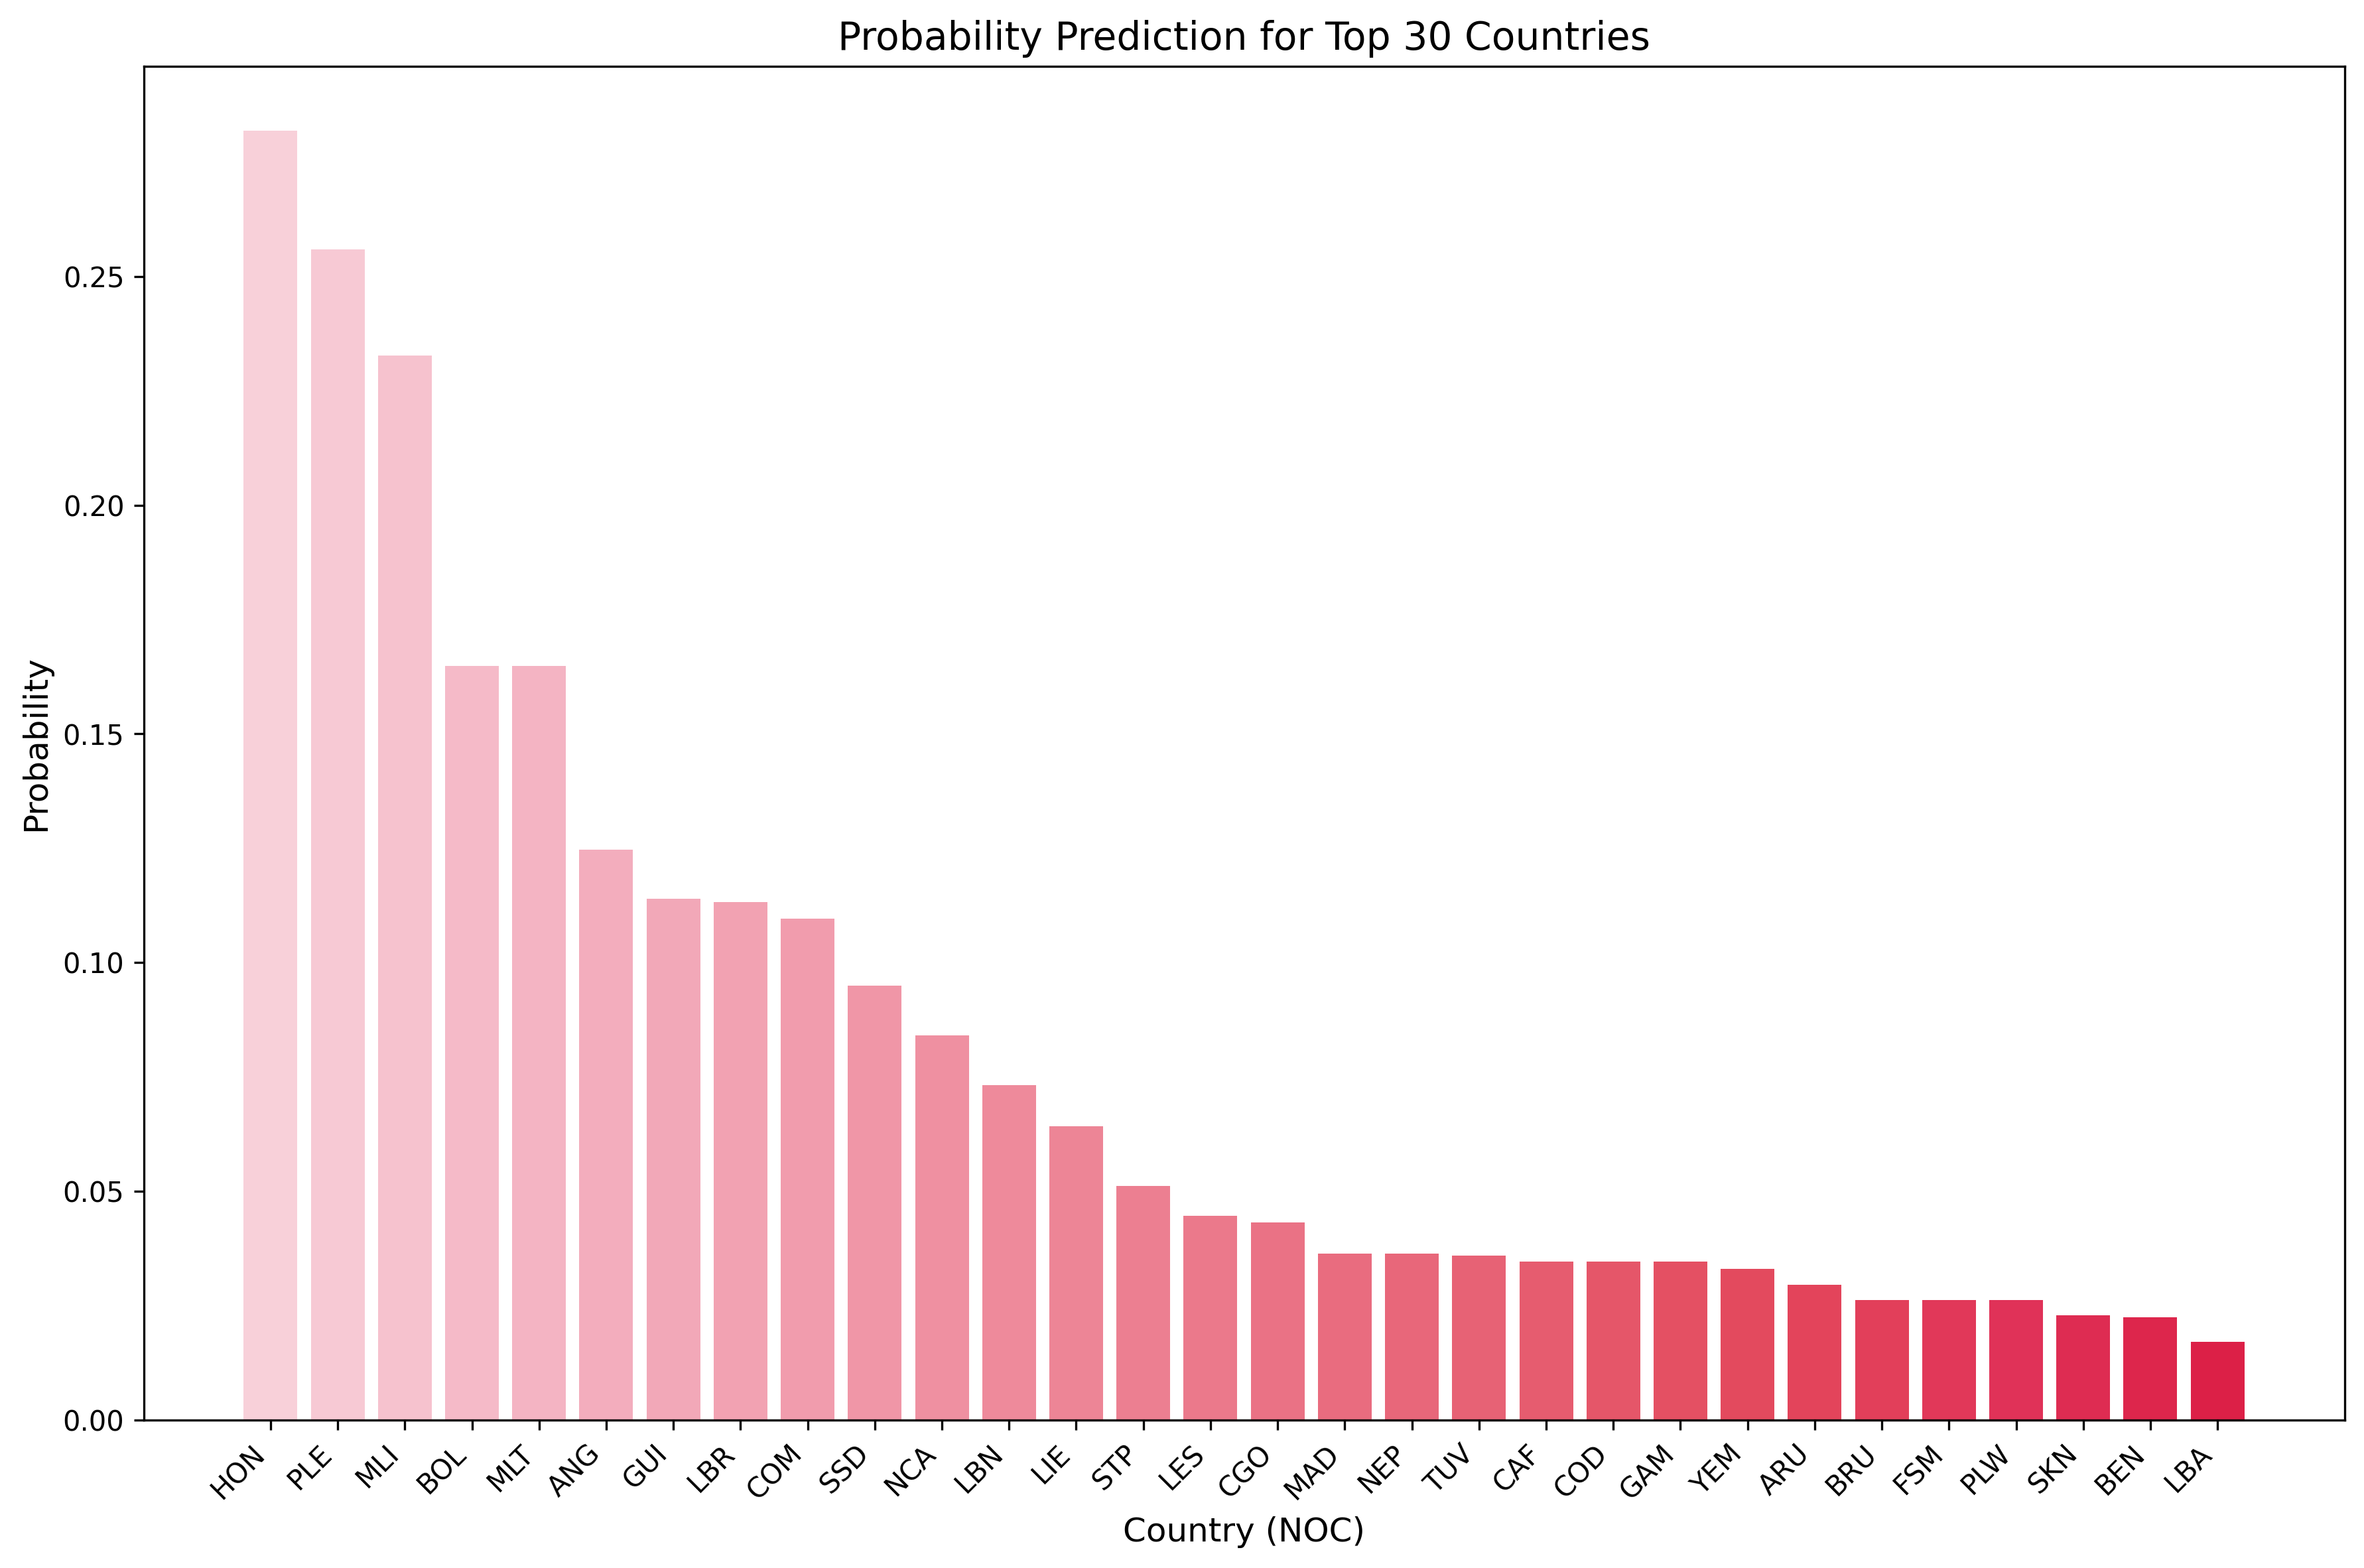
\includegraphics[width=0.6\linewidth]{Top30-Country-Probability-Prediction.png}
        \caption{Top30-Country-Probability-Prediction}
        \label{fig:enter-label}
    \end{figure}

    We assume the medal-winning probabilities for different countries are independent. The total probability distribution for $k$ countries winning medals is modeled using the binomial distribution. The binomial probability mass function is:
    \begin{equation}
        P(X = k) = \binom{N}{k} \prod_{i=1}^{N} p_i^{k_i} (1 - p_i)^{(1 - k_i)} \tag{17}
    \end{equation}
    where $X$ is the number of countries winning medals, $N$ is the total number of countries being considered, $k_i$ is 1 if country $i$ wins a medal and 0 otherwise, and $p_i$ is the predicted probability of country $i$ winning a medal. 

    Using Python, we computed the probability distribution of countries winning their first medal, as shown in Figure 6. Our prediction for the 2028 Los Angeles Olympics indicates that \textbf{two} countries have the highest probability, approximately \textbf{0.30}, of winning their first medal. Following them are one country with a probability of 0.28, three countries with a probability of 0.19, and zero countries with a probability of 0.12. Four countries have probabilities of 0.08, while the remaining scenarios have probabilities of less than 0.05, which are considered low-probability events.

    \begin{figure}[H]
        \centering
        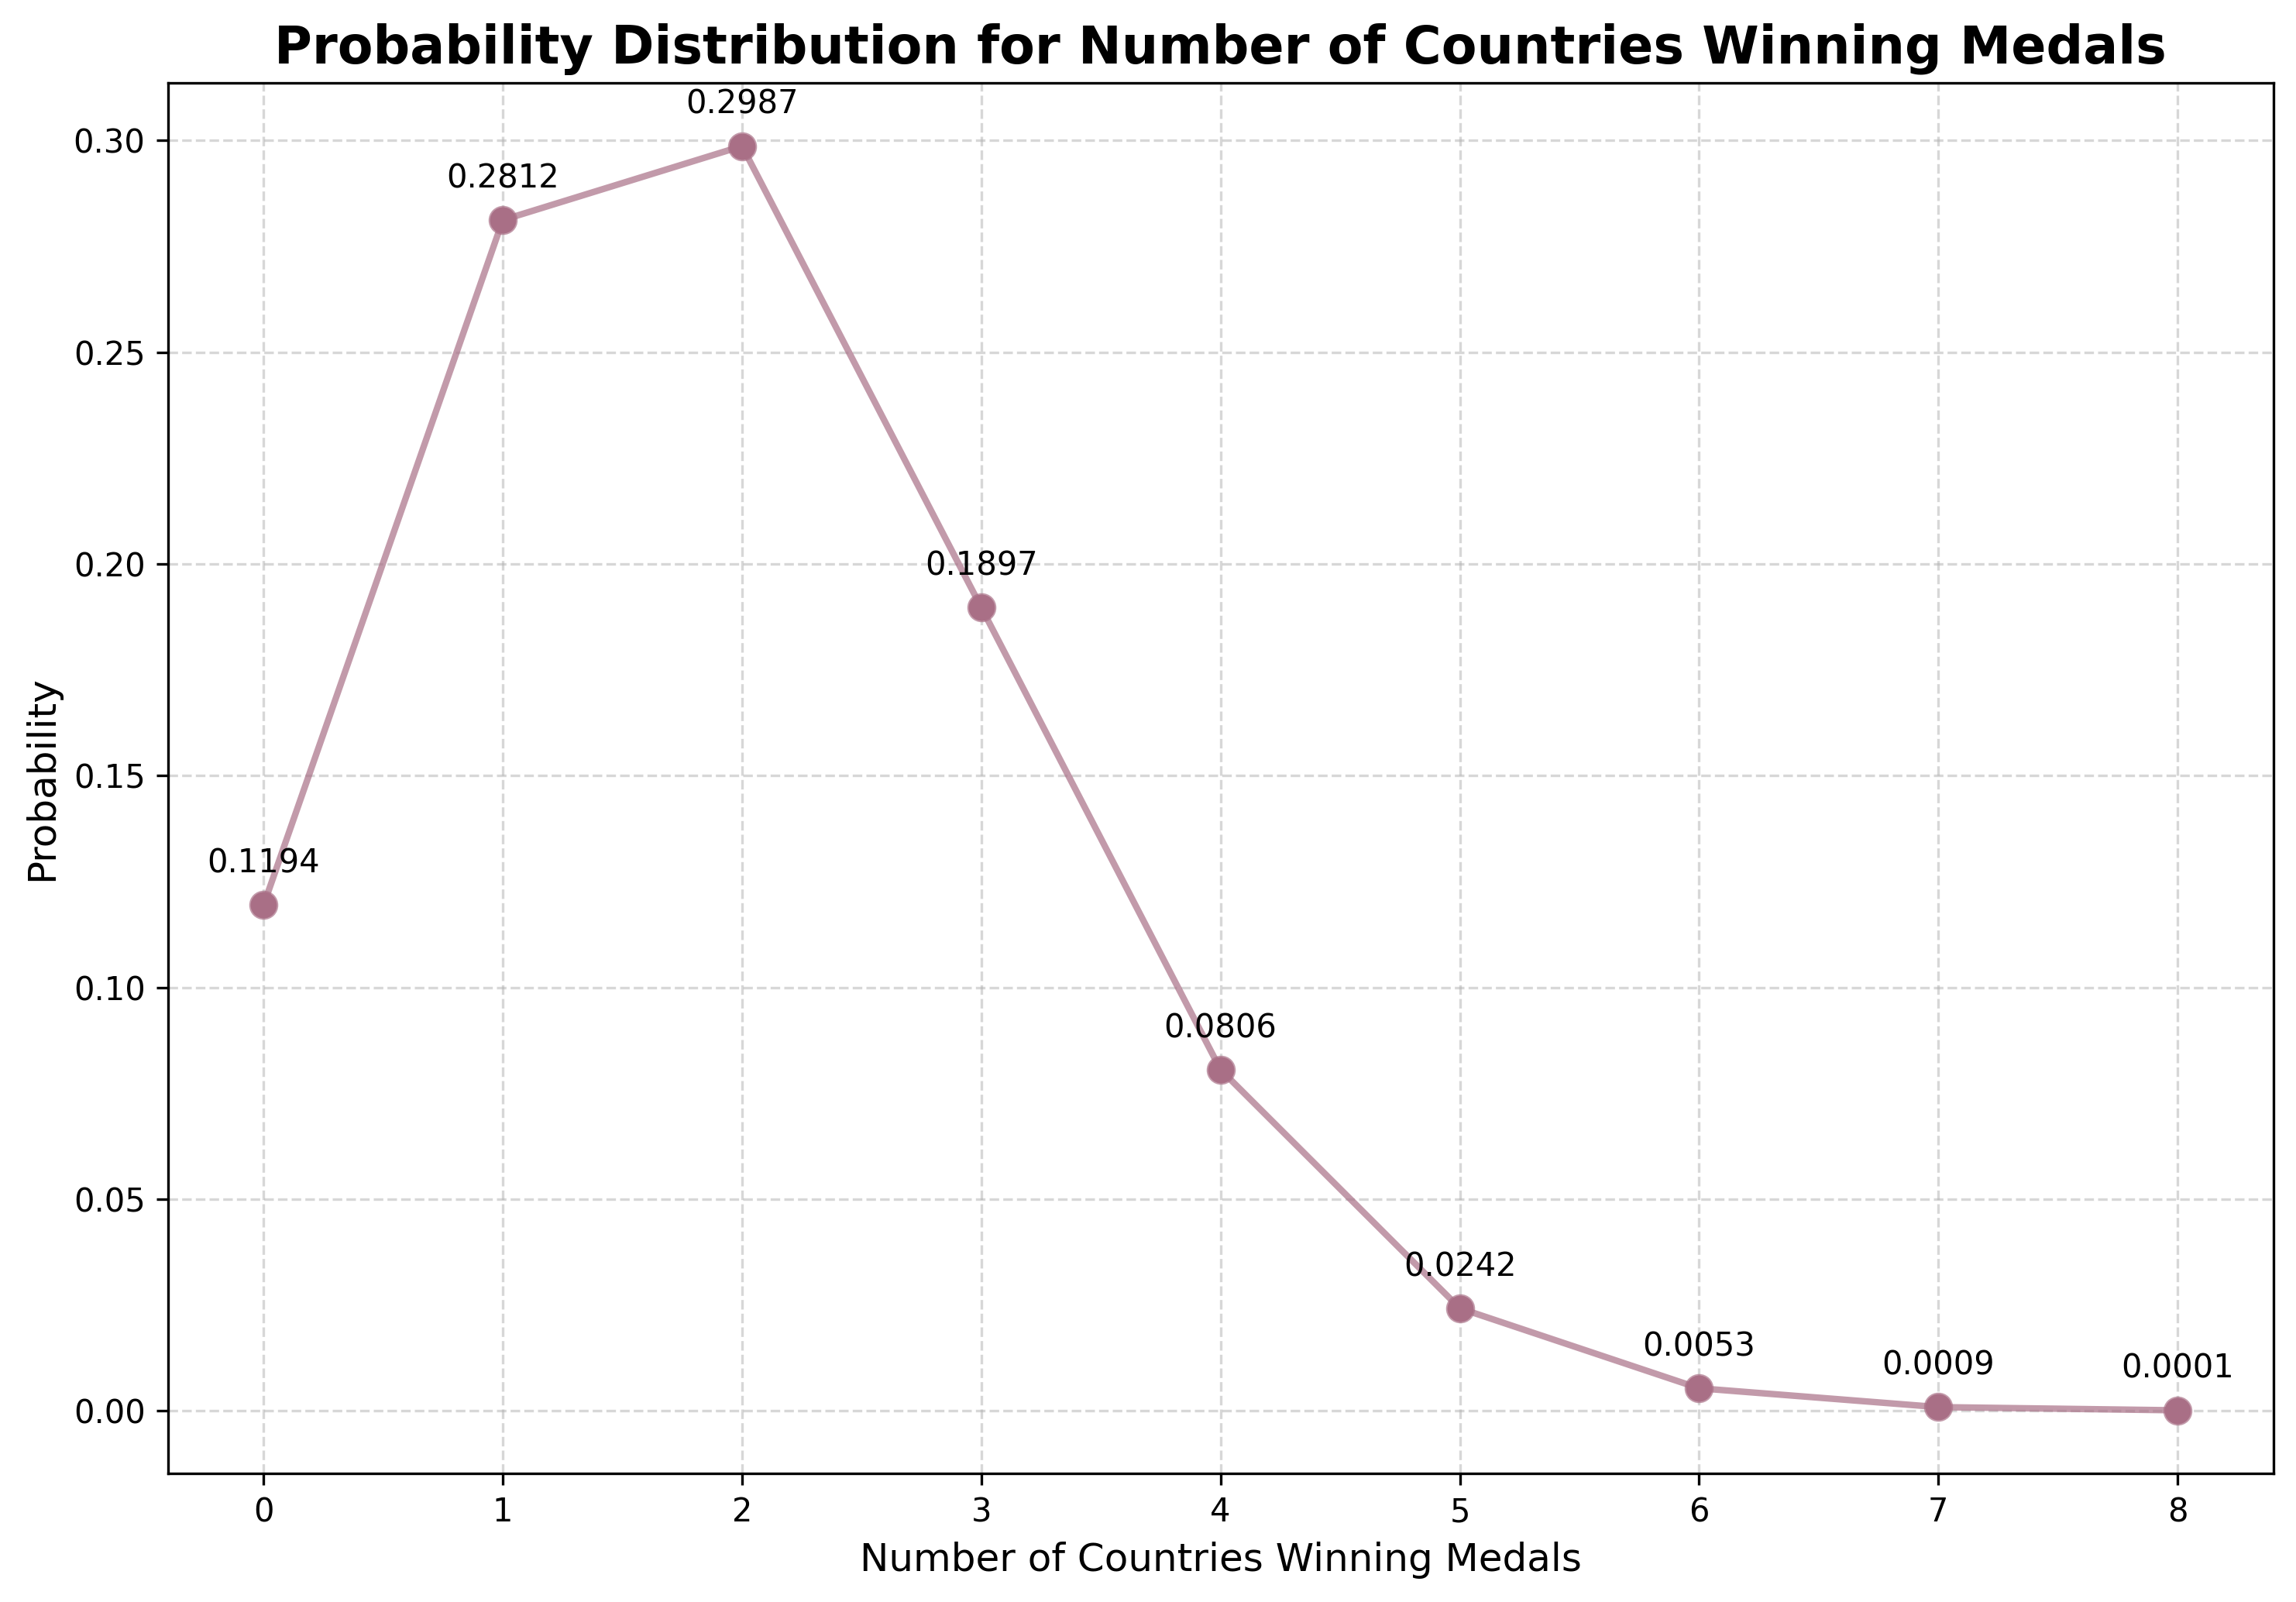
\includegraphics[width=0.75\linewidth]{Probability Distribution for Number of Countries Winning Medals.png}
        \caption{Probability Distribution for Number of Countries Winning Medals}
        \label{fig:enter-label}
    \end{figure}

\end{enumerate}

\section{Task 3: Exploring the Relationship Between Events and Medal Counts}
\subsection{Explore the Relationship of Events and Medal Counts}
The relationship between event types (both in terms of number and category) and medal counts is a fascinating area of research. To explore this, we conduct a statistical analysis on the number of athletes participating in various event types. Additionally, we create a correlation matrix to clearly visualize how the number of events and the event types contribute to the overall medal counts. This approach helps in identifying key patterns and understanding the factors influencing performance outcomes. There are numerous events, so we encoded different events and have only listed a few with full names as examples.
\begin{figure}[H]
        \centering
        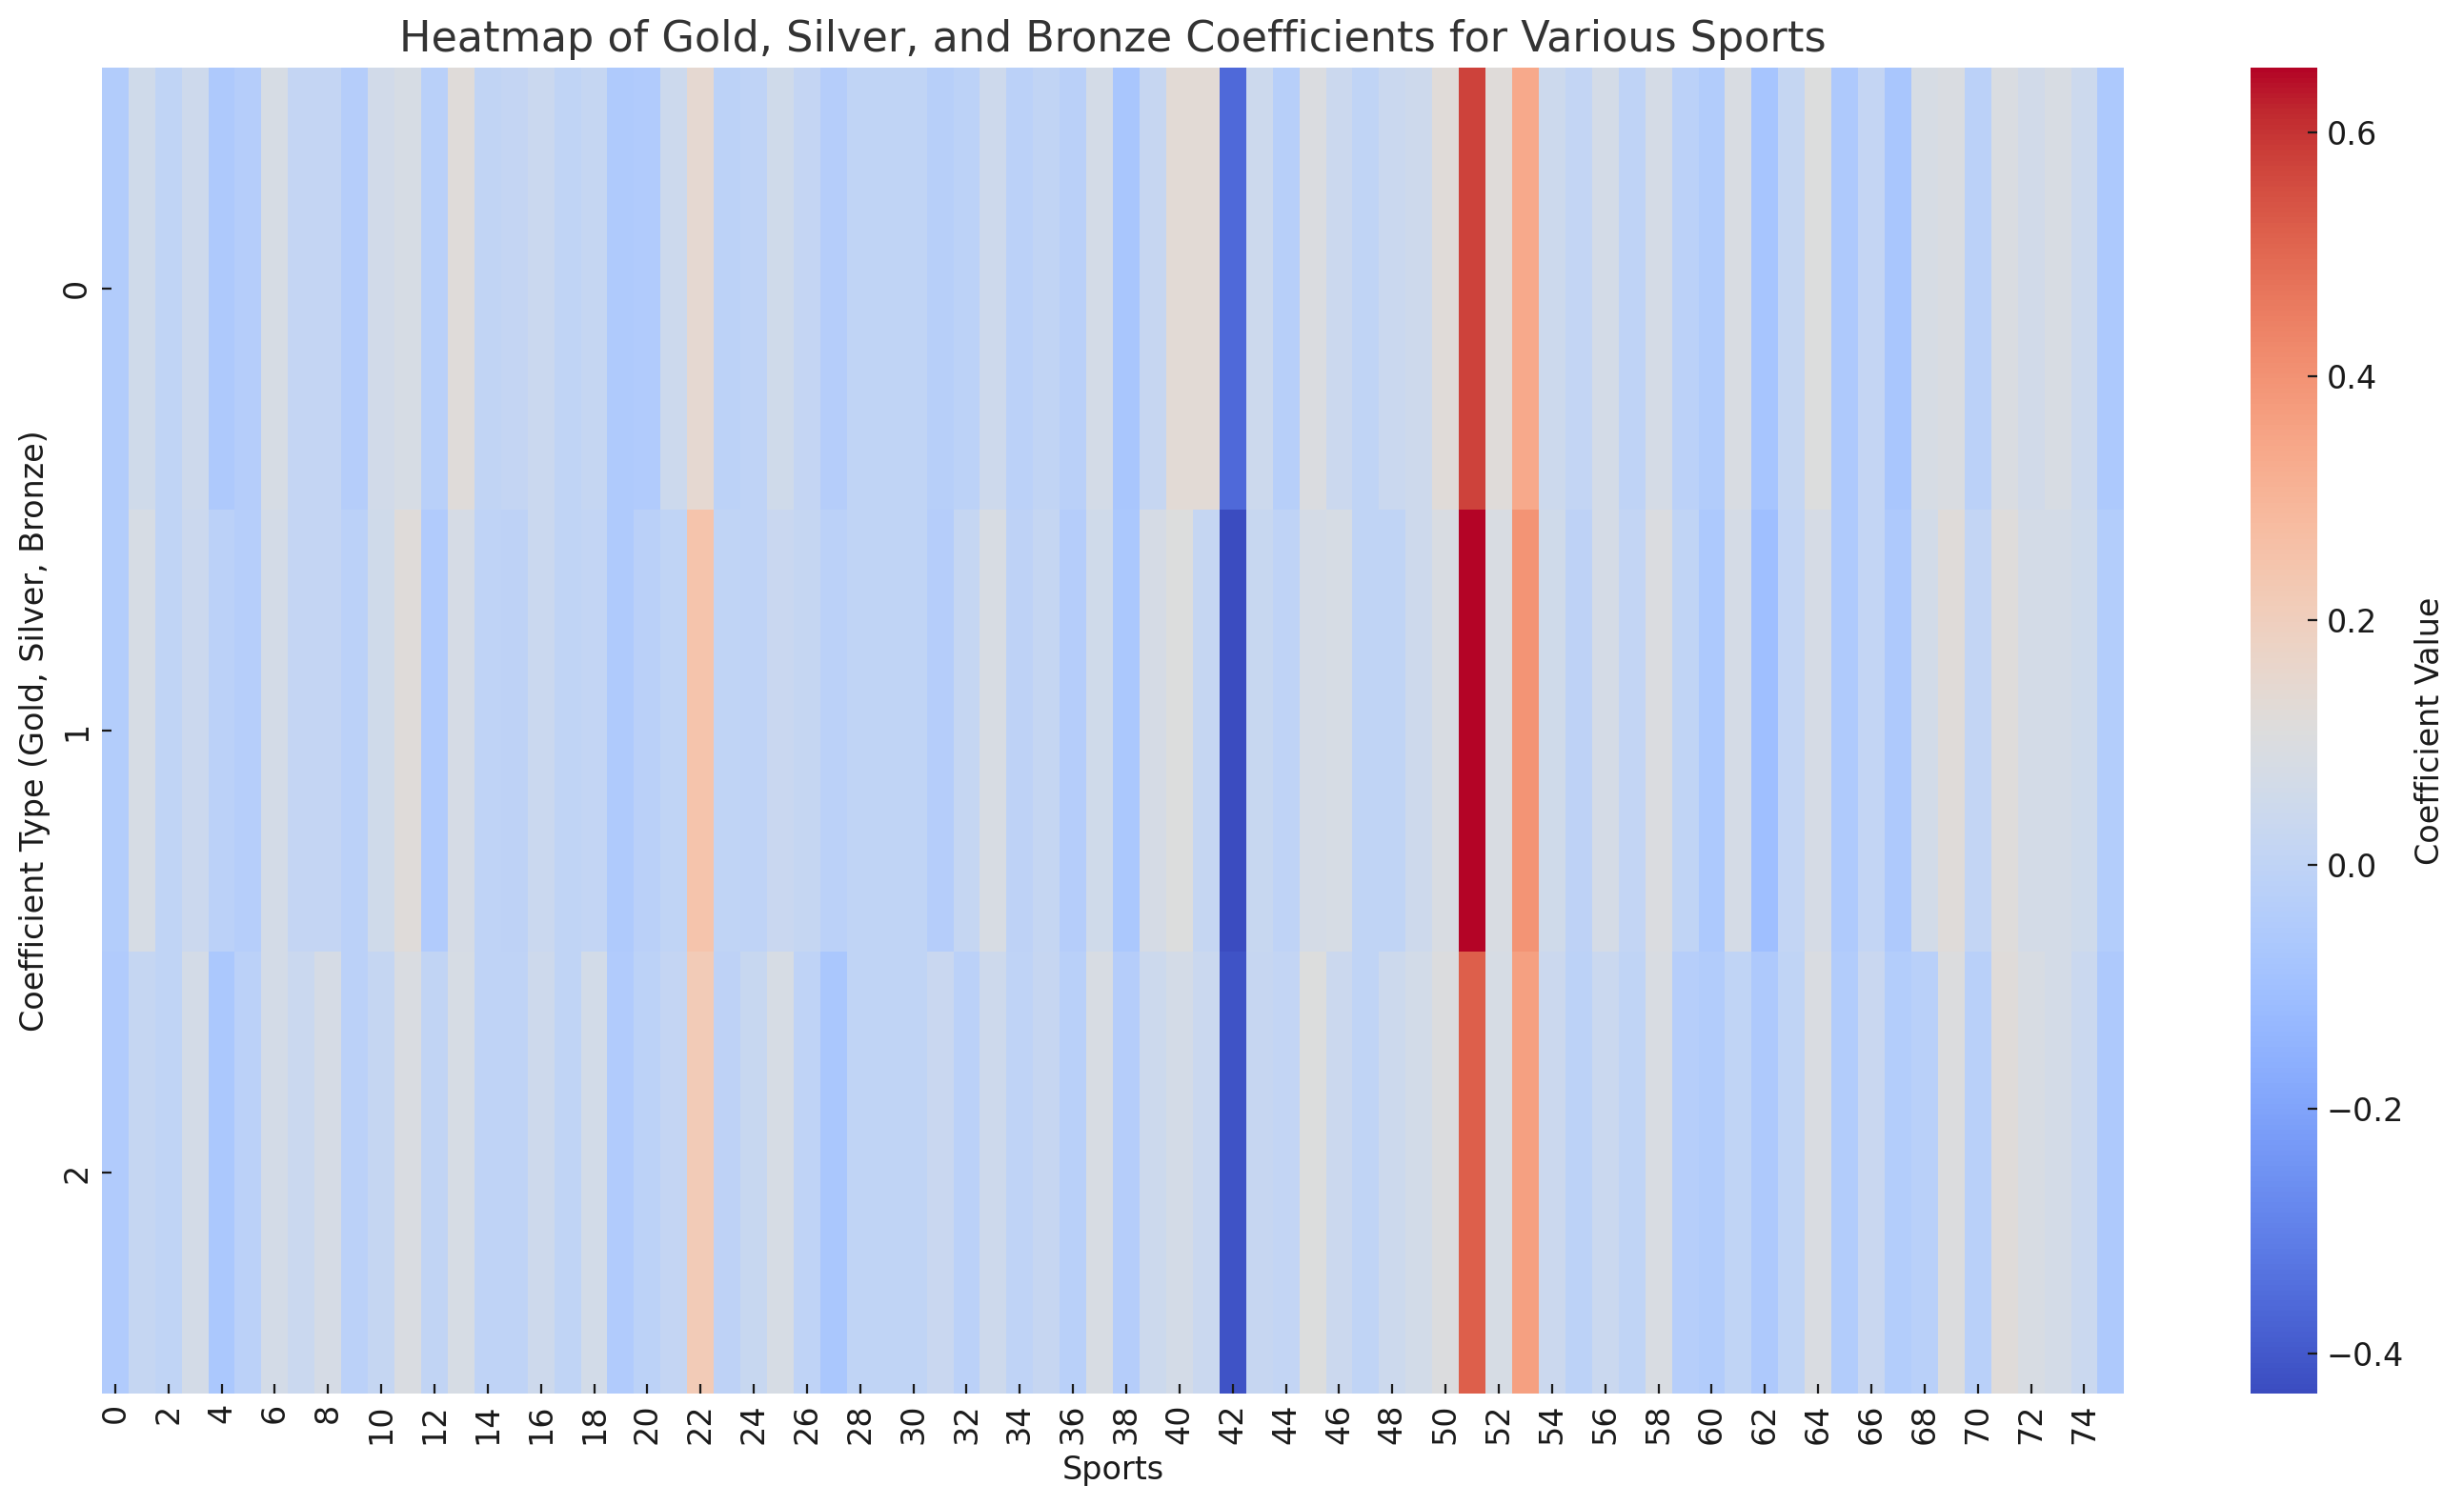
\includegraphics[width=0.75\linewidth]{Heatmap.png}
        \caption{Heatmap of Gold, Silver and Bronze Coefficients for Different Events }
        \label{fig:enter-label}
    \end{figure}
\begin{table}[ht]
\centering
\adjustbox{max width=\textwidth, valign=c}{ % Adjust the table to fit the width
\begin{tabular}{|l|r|r|r|r|r|r|r|r|r|r|r|r|r|}
\hline
Feature & Events & Sport\_3x3 Basketball & Sport\_3x3 Basketball, Basketball & Sport\_Aeronautics & Sport\_Alpinism & Sport\_Archery & Sport\_Art Competitions & Sport\_Artistic Gymnastics & Sport\_Artistic Swimming & \dots & Sport\_Wrestling \\
\hline
Golds Coefficients & -0.045377 & 0.058666 & 0.046575 & -0.057182 & -0.034728 & 0.081804 & 0.015434 & 0.01263 & -0.036921 & \dots & -0.060007 \\
\hline
Silvers Coefficients & -0.040295 & 0.081501 & 0.041639 & -0.015283 & -0.032828 & 0.069523 & 0.015134 & 0.015989 & -0.016273 & \dots & -0.039233 \\
\hline
Bronze Coefficients & -0.047274 & 0.019216 & 0.070082 & -0.067294 & -0.016598 & 0.07101 & 0.035957 & 0.078456 & -0.015647 & \dots & -0.058405 \\
\hline
\end{tabular}
}
\caption{Coefficients Matrix}
\end{table}
We can observe that different events may have varying positive or negative effects on medal counts, for example, 3x3 Basketball has a positive effect on medal counts while Artistic Swimming has a negative effect on medal counts

\subsection{The Importance of Sports Projects for a Country}
A country's investment and emphasis on sports significantly influence the number of athletes and their overall performance\cite{10}. To identify the most important Olympic sports for a country, we must analyze both the number of athletes participating and the country's achievements in each sport.

\subsubsection{Data Normalization and Proportional Analysis}
However, the inherent differences between sports, the number of participants and the total number of medals available,must be taken into account. For example, in 2024, the athletics event had 1810 participants and 144 medals, while table tennis had only 172 participants and 15 medals.
To eliminate the influence of these differences between sports, we process the data as follows:
For each country, we calculate the proportion of participation and medal achievements in each sport. Specifically, the participation ratio for each event is defined as:
\begin{equation}
    \text{PAratio}_{i,j} = \frac{\text{PA}_{i,j}}{\sum_i \text{PA}_{i,j}} \tag{18}
\end{equation}
where $PA_{i,j}$ represents the total number of athletes from country $i$ in sport $j$.

Similarly, we compute the PE for each sport in each country using the previously mentioned Fibonacci Weighted Point System. The performance ratio for each event is: 
\begin{equation}
    PE_{\text{ratio},i,j} = \frac{PE_{i,j}}{\sum_{i=1}^{N} PE_{i,j}} \tag{19}
\end{equation}
where N is the number of countries.

\subsubsection{Entropy Weight Method (EWM)}
To determine the relative importance of participation ratio and performance ratio, we use the EWM. This method allows us to quantify the relative importance of each feature (participation and performance) in assessing the importance of each sport. $H_j$: The entropy for feature $j$ is computed as follows:
\begin{equation}
    H_j = -\frac{1}{\ln(N)} \sum_i P_{i,j} \ln(P_{i,j}) \tag{20}
\end{equation}

where where $P_{i,j}$ is the normalized value of feature $j$, and $N$ is the number of countries.

The weight for each feature $j$ is then derived using the following formula:
\begin{equation}
    W_j = \frac{1 - H_j}{\sum_{j=1}^{M} (1 - H_j)}\tag{21}
\end{equation}
where $M$ is the number of features. 

\subsubsection{TOPSIS Method}
Once the weights for the participation ratio and performance ratio are determined, we apply the TOPSIS method to calculate the overall importance score for each sport. The steps of the TOPSIS method are as follows:
\begin{enumerate}[\textbullet]
    \item \textbf{Step 1: Construct and Normalized Decision Matrix:} We construct a decision matrix where each row represents a country and each column represents a specific sport. Each element $x_{ij}$ in this matrix corresponds to the combined value of participation and performance ratios for country $i$ in sport $j$.

    In order to eliminate the influence of different dimensions of indices, we standardize the matrix. The standardization formula is as follows:
    \begin{equation}
        z_{ij} = \frac{x_{ij}}{\sqrt{\sum_{i=1}^{n} x_{ij}^2}}\tag{22}
    \end{equation}
    Use $Z_{ij}$ as the element to construct the normalized matrix $Z_{n×m}=[Z_{ij}],i=1,...,n; j=1,...,m;$
    
    \item \textbf{Step 2: determine the best and worst solutions:} For each column (representing a sport), we determine the best and worst solutions:

    The best solution $Z^+$ is the maximum value for each column:
    \begin{equation}
        Z^+=(max(Z_{i1}),max(Z_{i2}),...,max(Z_{im})\tag{23}
    \end{equation}
    The worst solution $Z^-$ is the minimum value for each column:
    \begin{equation}
        Z^-=(min(Z_{i1}),min(Z_{i2}),...,min(Z_{im})\tag{24}
    \end{equation}
    Calculate the distance between $Z^+$ and $D_i^+$ and the distance between $Z^-$ and $D_i^-$ for each evaluation object. The calculation of the distance here needs to use the weight calculated by the EWM method in the previous section.
    \begin{equation}
        D_i^+ = \sqrt{\sum_{j=1}^{m} w_j (\max Z_{ij} - Z_{ij})^2} \quad \quad D_i^- = \sqrt{\sum_{j=1}^{m} w_j (\min Z_{ij} - Z_{ij})^2}\tag{25}
    \end{equation}

    \item \textbf{Step 3: Calculate the Closeness Index:  } 
    
    \begin{equation}
        C_i = \frac{D_i}{D_i^+ + D_i^-} \quad 0 \leq C_i \leq 1\tag{26}
    \end{equation}
    
    The closer $C_i$ is to 1, the more important sport $j$ is for country $i$. A higher $C_i$ value indicates that sport $j$ is of more importance to that country.

    \item \textbf{Results}
    To illustrate the application of our model, we focused on China (CHN) and input the normalized participation and performance ratios for each sport into the model. These ratios, derived from China’s historical athlete participation and medal achievements, were processed using the \textbf{EWM-TOPSIS Model} to calculate the Closeness Index for each sport. This index represents the proximity of each sport’s performance to the optimal solution, with higher values indicating greater importance.

    As shown in the Figure 8 below, the Closeness Index for \textbf{table tennis (Closeness = 0.90)} is the highest among all sports, underscoring its paramount importance to China in the Olympic context. Following closely are badminton,trampolining, and diving, all of which have Closeness values exceeding \textbf{0.5}. These sports are also critical to China’s Olympic strategy, highlighting their significant role in the country’s athletic achievements.
\end{enumerate}

\begin{figure}[H]
    \centering
    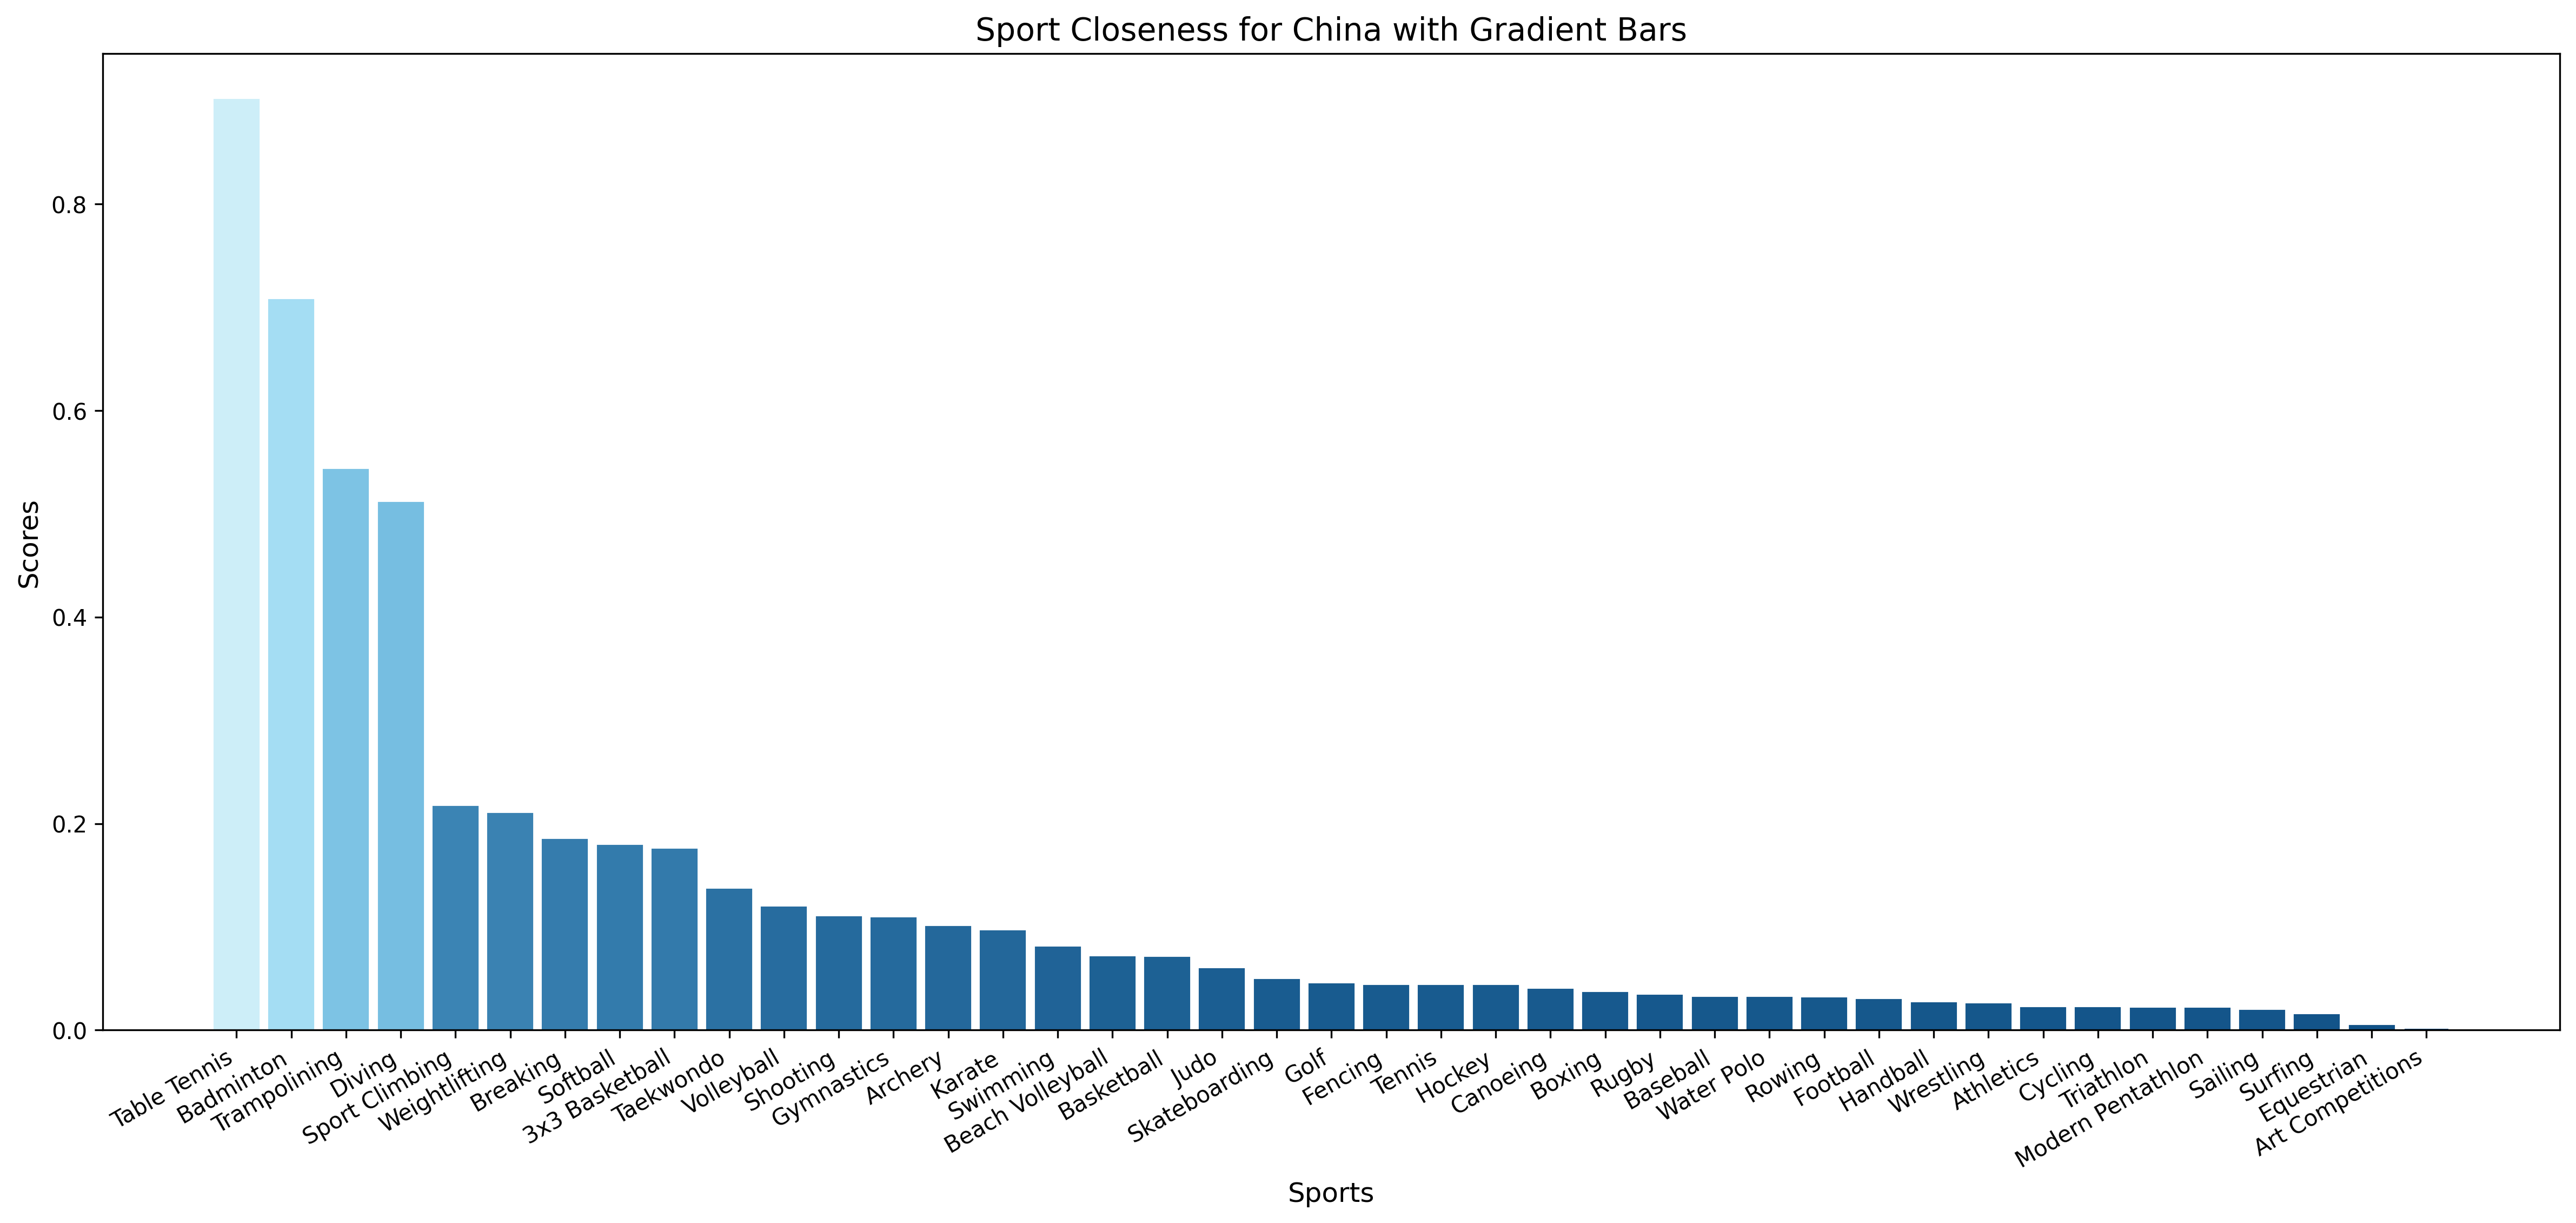
\includegraphics[width=0.75\linewidth]{Sport-Score-CHN.png}
    \caption{Sport Closeness for China with Gradient Bars}
    \label{fig:enter-label}
\end{figure}

\subsection{Analysis of the Impact of New Olympic Events on Host Country Performance}

In most Olympic Games, new events are introduced either to promote the development of a specific sport or at the discretion of the host country to encourage the popularity of certain activities. The objective of this analysis is to evaluate the impact of these new events on the performance of athletes from the host country, by comparing the per capita performance of host country athletes with that of all athletes.

\begin{enumerate}[\textbullet]
    \item \textbf{Step 1: Quantification of Performance}
    
    To account for the incomplete nature of early Olympic Games, which introduced many new events, we focus on data from the Games held after 1964. The performance of athletes is quantified as follows:
    \[
    PE_h = \frac{1}{n} \sum_{i=1}^{n} PE_{ij} \tag{27}
    \]
    where \( PE_{ij} \) represents the performance score of the $i^{th}$ athlete in the $j^{th}$ event, and \( n \) is the total number of athletes.
    $PE_o$: Per capita performance score of all athletes, calculated in the same way as for the host country.

    As shown in Figure 9, the differences in performance between the host countries and all athletes vary across different Olympic Games.

    \item \textbf{Step 2: Mann-Whitney U Test}

    To evaluate whether there is a significant difference between the performance of host country athletes in new events and that of all athletes, we applied the \textbf{Mann-Whitney U Test}, also known as the \textbf{Wilcoxon Rank-Sum Test}\cite{11}. This non-parametric test is suitable for small sample sizes and non-normally distributed data, and it has been shown to be effective (K. V. Mardia)\cite{12}.

    \textbf{Our Hypotheses:}
    
    \textbf{Null hypothesis ($H_0$):} The per capita performance of host country athletes is equal to that of all athletes, i.e., \(PE_{host} = PE_{all}\).
    
    \textbf{Alternative hypothesis ($H_1$):} The per capita performance of host country athletes is not equal to that of all athletes, i.e., \(PE_{host} \neq PE_{all}\).
    
    The Mann-Whitney U test statistic is computed as follows:
    \[
    U = n_1n_2 + \frac{n_1(n_1+1)}{2} - R_1 \tag{28}
    \]
    where \(n_1\) and \(n_2\) represent the sample sizes of the two groups, and \(R_1\) is the sum of ranks for the host country athletes.

    Using Python, the Mann-Whitney U test statistic was computed to be \textbf{47.0}, with a p-value of \textbf{0.596}.

    \item \textbf{Result Analysis}
    
    Given that the p-value is greater than 0.05, we fail to reject the null hypothesis. This suggests that there is no statistically significant difference between the per capita performance of host country athletes and that of all athletes in the new events. This finding aligns with the conclusions of Gergely Csurilla, who reported no significant effect of hosting on athlete performance\cite{13}.
\end{enumerate}

 \begin{figure}[h]
        \centering
        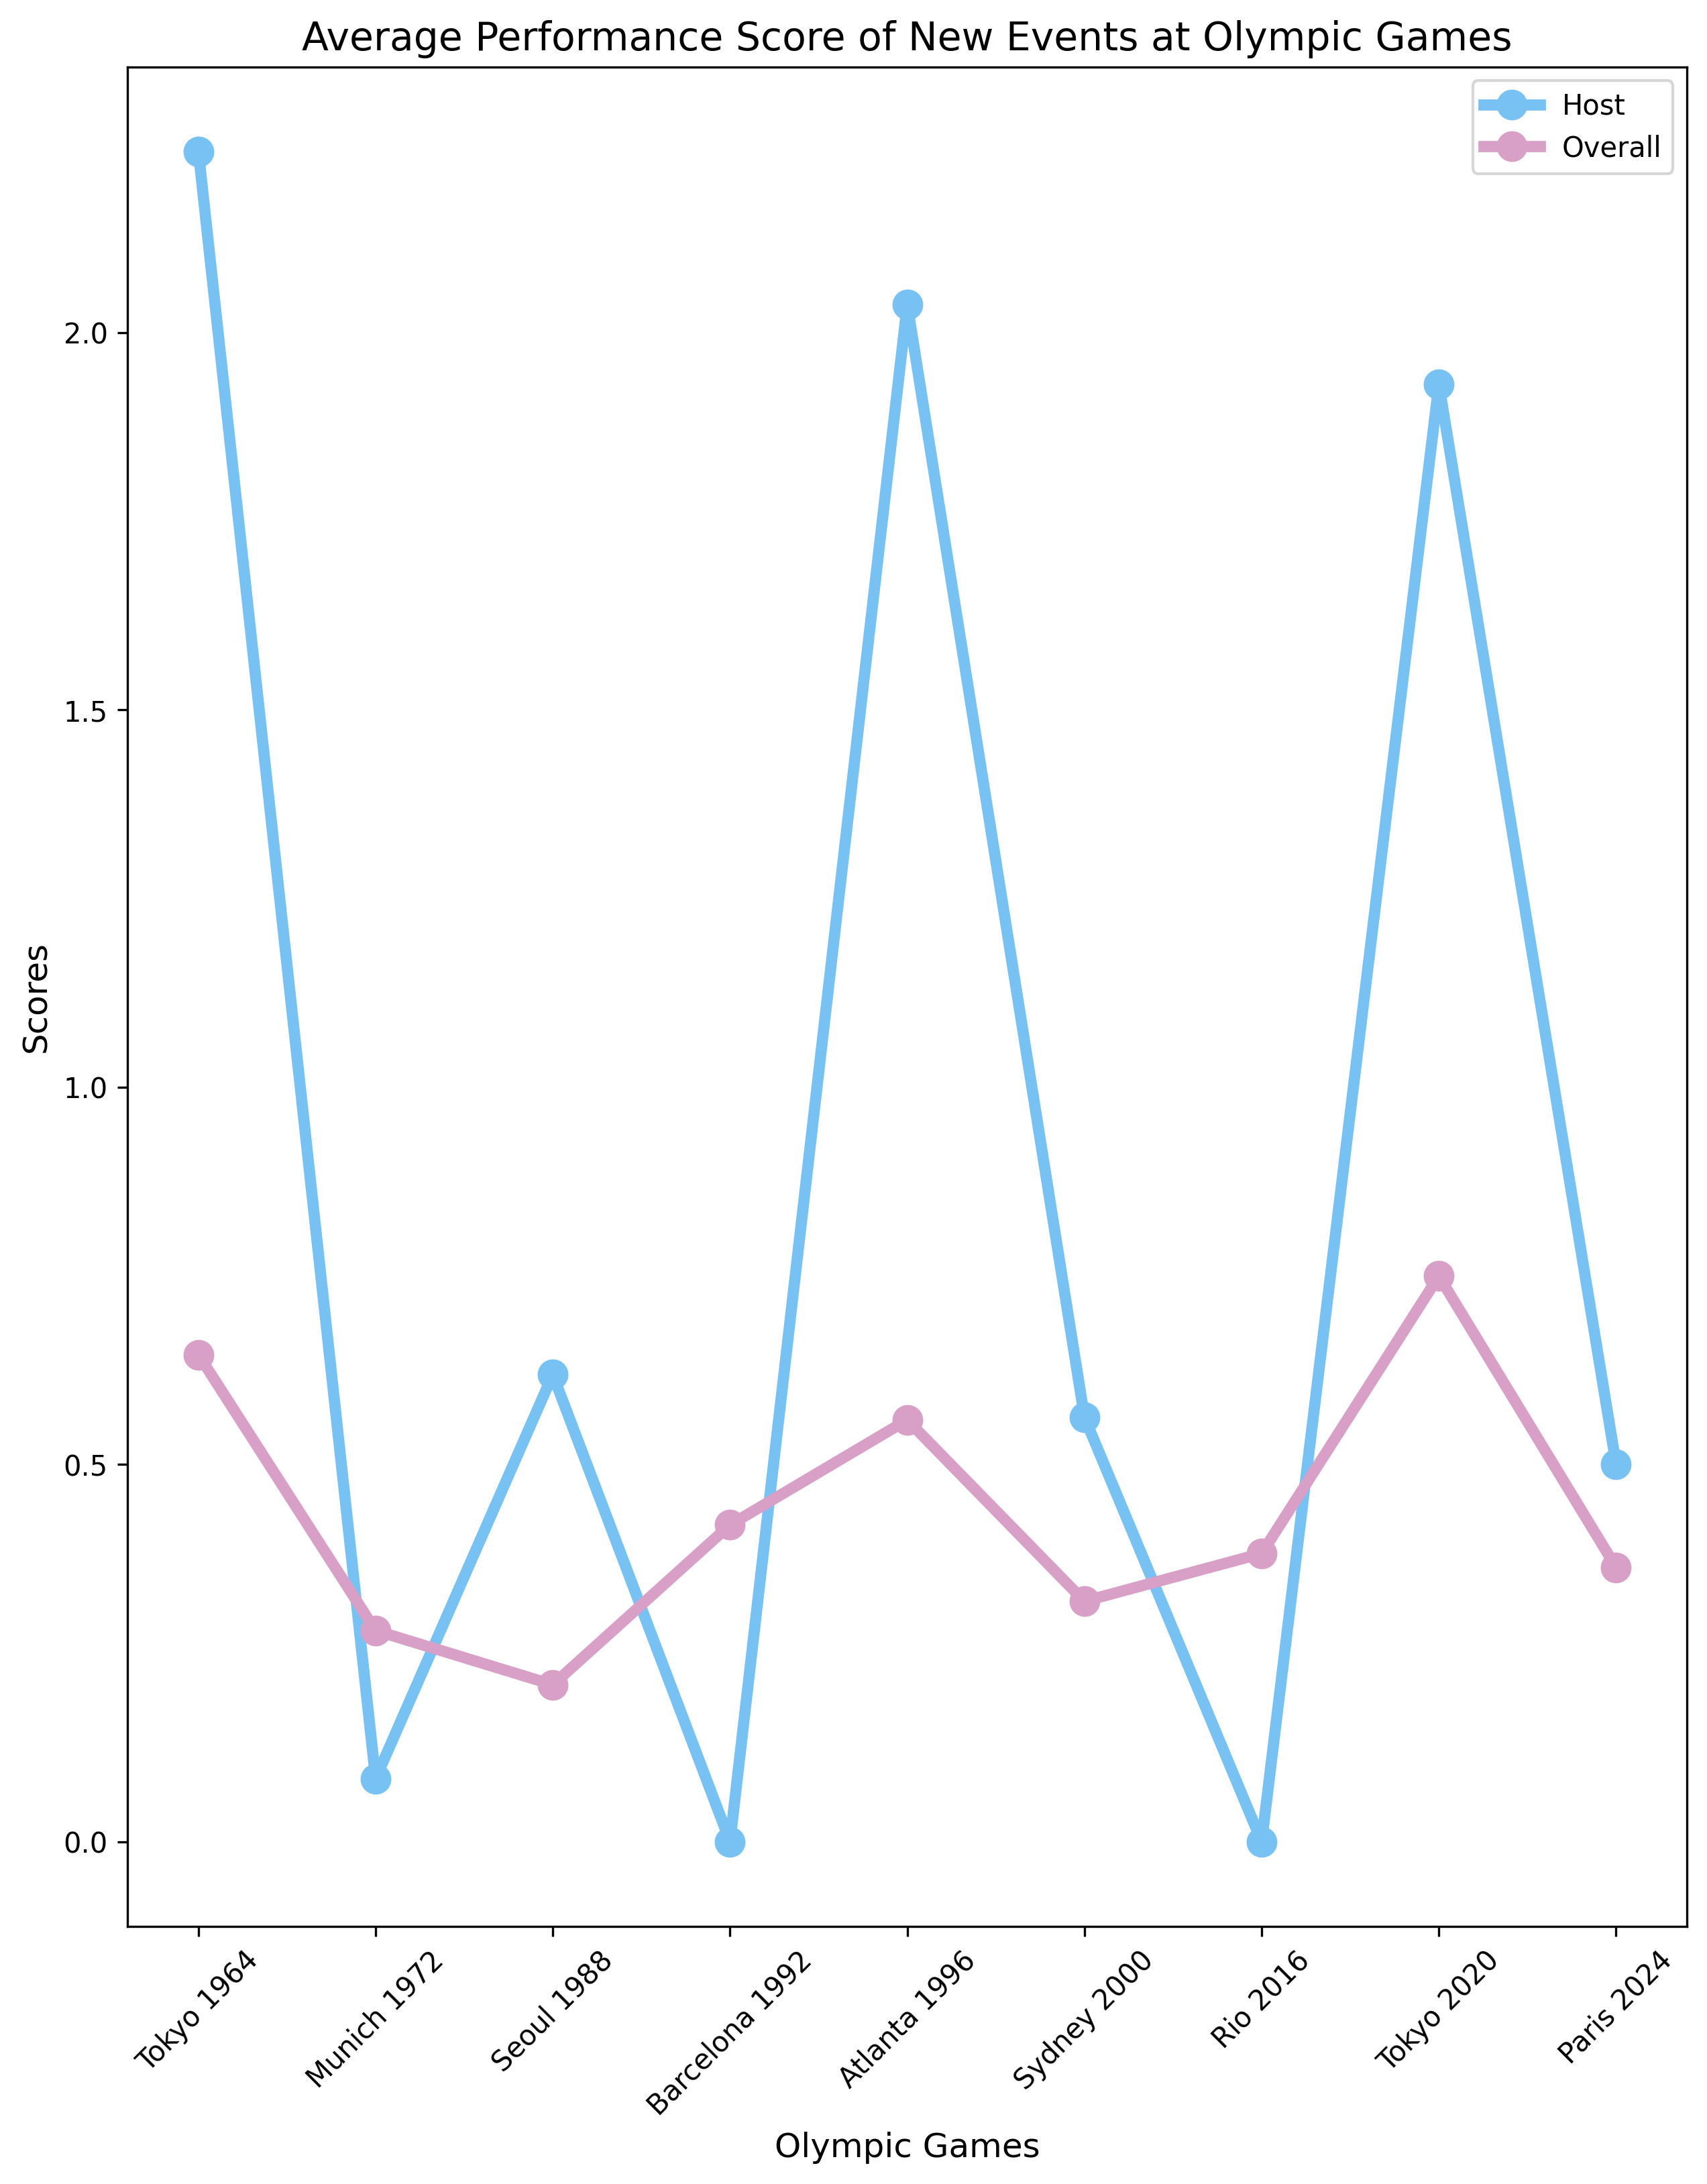
\includegraphics[width=0.5\linewidth]{Performance-Scores-Over-Olympic-Games.png}
        \caption{Average Performance Score of New Events at Olympic Games}
        \label{fig:enter-label}
    \end{figure}


\section{Task 4: Evaluating the "Great Coach" Effect}
\subsection{Evidence for the existence of the "great coach" effect}
The "great coach" effect is evident in the careers of Lang Ping and Béla Károlyi. Lang Ping led both Chinese and American volleyball teams to championships, showcasing her adaptability across cultures. Similarly, Béla Károlyi guided Romanian and American gymnastics teams to success, proving exceptional coaching transcends boundaries. Data analysis highlights Károlyi’s significant impact on the USA team’s performance in the 2016 Olympics, with results surpassing predicted medal counts, emphasizing his coaching influence.
\begin{table}[h!]
\centering
\begin{tabular}{lcccc}
\toprule
\textbf{} & \textbf{Gold} & \textbf{Silver} & \textbf{Bronze} & \textbf{Total} \\
\midrule
Predicted & 45 & 35 & 31 & 111 \\
Actual    & 46 & 37 & 38 & 121 \\
\bottomrule
\end{tabular}
\caption{Comparison of Predicted and Actual Medal Counts for the USA in the 2016 Olympics}
\label{tab:usa_medals_2016}
\end{table}







\subsection{Anticipating the effect's contribution to medal counts}

To better evaluate the effect, we continue to use $PE_i=3g_i+2s_i+b_i$ to quantify performance\cite{3}. Using the Fibonacci Weighted Point System in conjunction with the collected data, we estimate that the influence of the exceptional coaching effect increases medal counts by approximately 10\%. This calculation highlights the significant role of coaching expertise in enhancing team performance and surpassing predicted outcomes.
\subsection{Suggestions for three countries to make use of such effect}


\begin{enumerate}[\textbullet]
    \item \textbf{India – Athletics (Track & Field and Middle/Long Distance Running):}
    India has potential in athletics but struggles in track and field beyond Neeraj Chopra's 2020 javelin gold. To improve, India could hire top international coaches in sprinting (e.g., from Jamaica or the US) and distance running (e.g., Ethiopia or Kenya), invest in youth development, and establish world-class training facilities. A focused strategy with expert coaching could boost India's competitiveness and medal prospects in future global events.

    \item \textbf{Brazil – Swimming:}
    Brazil excels in team sports but has untapped swimming potential, despite talents like César Cielo. Hiring elite coaches from the US or Australia and focusing on youth development through long-term training programs could deepen its talent pool. With world-class guidance, Brazil could strengthen its global presence in swimming.

    \item \textbf{South Africa – Boxing:}
   South Africa, with its boxing history and potential, can regain prominence in lightweight and welterweight categories by hiring renowned coaches from Cuba or Eastern Europe, known for rigorous training systems. Strategic investment in coaching and grassroots programs could boost Olympic success and medal counts.
\end{enumerate}

\section{Task 5: Proposing a Unique Insight Into the Olympic medal}
In \textbf{Task 2}, our model focuses on identifying patterns for countries that have never won a medal but are poised to win their first medal. \textbf{Task 3} investigates the relationship between sports and the number of medals won by countries. In \textbf{Task 4}, we emphasize the influence of great coaches and made recommendations for three countries. Together, these tasks lead us to the following key question: Can we leverage historical data to determine which sports are most suitable for countries to win their first medal? Furthermore, can we use the historical data of countries that have never won a medal to recommend specific sports for them to focus on, helping them secure their first Olympic medal by 2028?

\begin{enumerate}[\textbullet]
    \item \textbf{Step 1: Data Processing: }
    We begin by analyzing athlete data to identify the sports in which each country won its first medal. Each sport is then scored based on the following formula, derived from the Fibonacci sequence: 
    \begin{equation}
        S_i = 3a_i +2b_i +c_i\tag{29}
    \end{equation}
    $a_i$, $b_i$, and $c_i$ represent the number of gold, silver, and bronze medals, respectively, in the $i^{th}$ sport.
    
    Based on this scoring system, the sports most suitable for countries to win their first medal are identified. For example,\textbf{ Athletics (119)}, \textbf{Wrestling (44)}, \textbf{Shooting (38)}, and \textbf{Boxing (37)} are the top sports with the highest scores.

    \begin{figure}[h]
        \centering
        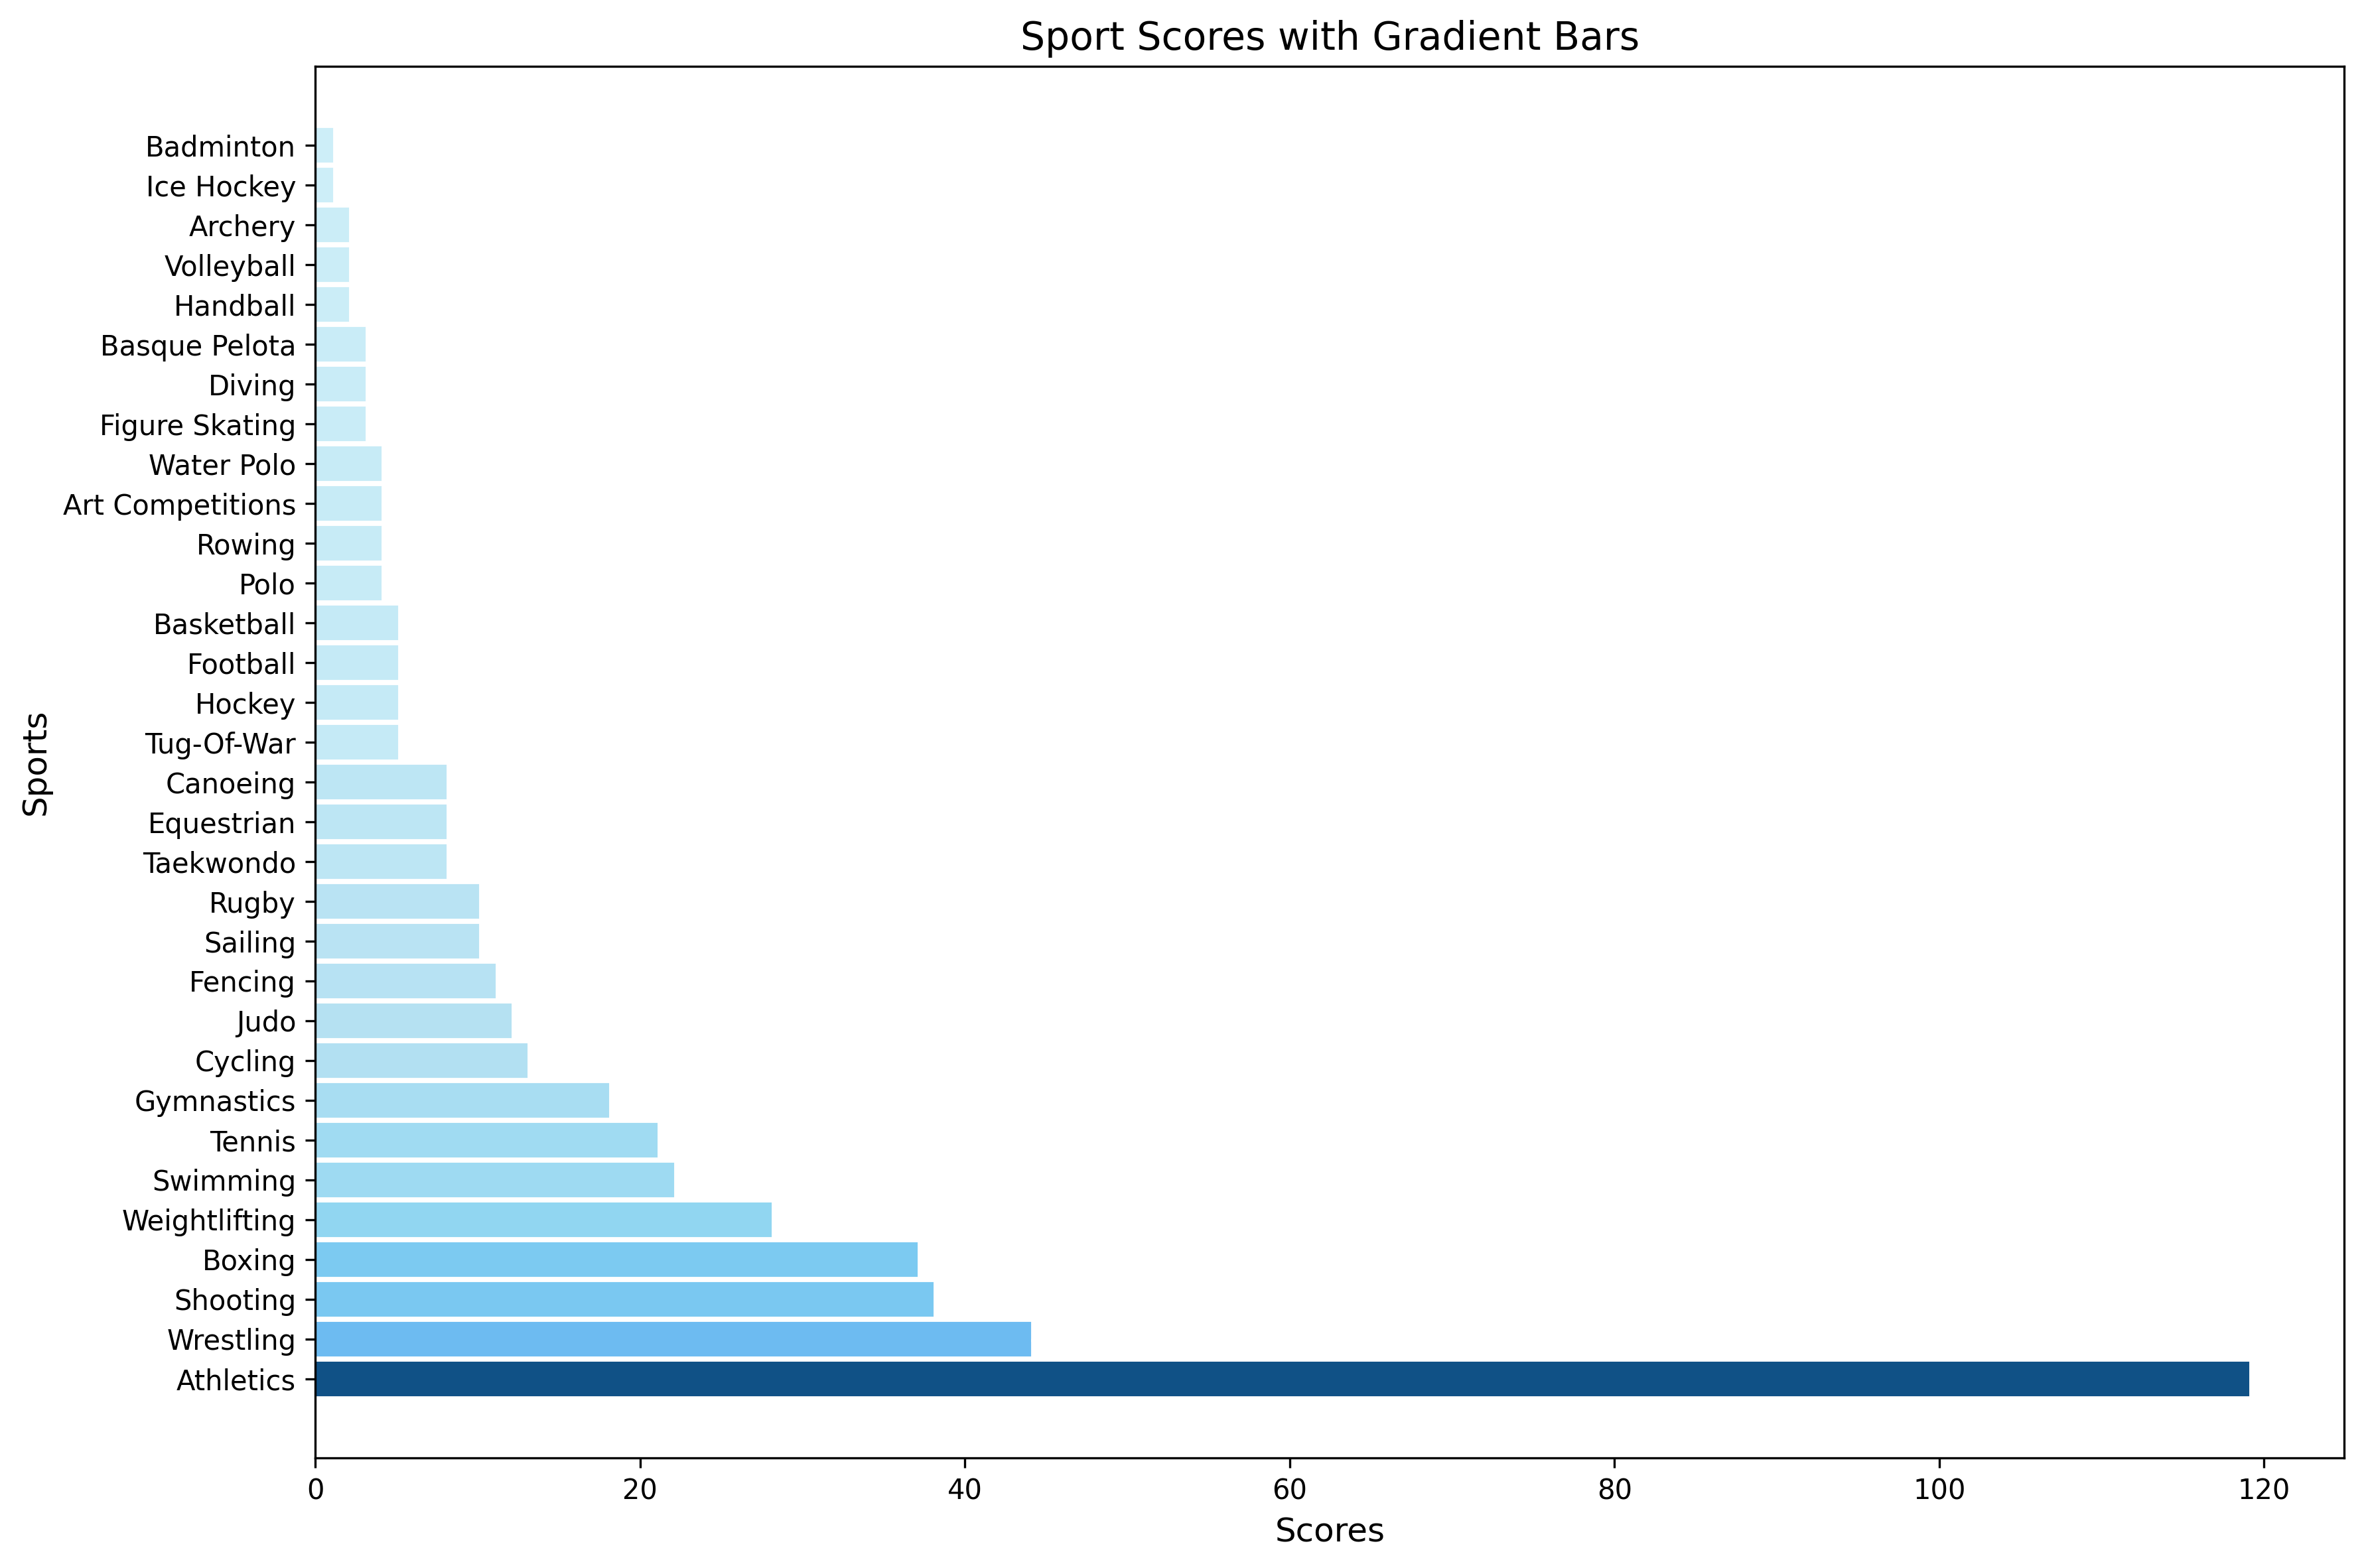
\includegraphics[width=0.75\linewidth]{Sport-Score2.png}
        \caption{Sport Scores with Gradient Bars}
        \label{fig:enter-label}
    \end{figure}

    \item \textbf{Step 2: Building recommendation equation: }Next, we calculate the number of times each country has participated in each sport. Finally, by integrating the sport scores and the historical participation data of each country, we use XGBoost to predict the probability of each country winning its first medal in the 2028 Olympics. This results in the following recommendation equation:
    \begin{equation}
        P_{\text{Medal},i,p,2028} = \sigma \left( \beta_0 + \beta_1 \cdot S_p + \beta_2 \cdot C_{i,p} + \beta_3 \cdot (S_p \cdot C_{i,p}) \right)\tag{30}
    \end{equation}

    The probability $P_{\text{Medal}, i, p, 2028}$ represents the likelihood that country $i$ wins a medal in sport $p$ in the 2028 Olympics. The sport score $S_p$ is calculated using the Fibonacci-based formula, while $C_{i,p}$ denotes the number of times country $i$ has participated in sport $p$. The model parameters $\beta_0,\beta_1,\beta_2,\beta_3$ are learned during training. The Sigmoid function $\sigma(x) = \frac{1}{1 + e^{-x}}$ is then applied to map the prediction to a probability in the range [0, 1].

    \item \textbf{Step 3: Results: }Based on the highest $P_{\text{Medal}, i, p, 2028}$, we identify the leading countries for each sport. We recommend the following target sports for Olympic preparation: \textbf{Boxing} for the Myanmar Olympic Committee (MYA), \textbf{Shooting} for the Malta Olympic Committee (MLT), \textbf{Athletics} for the Mali Olympic Committee (MLI), and \textbf{Wrestling} for the Gambia Olympic Committee (GBS).

    
\end{enumerate}






\section{Sensitivity Analysis}
A sensitivity analysis of the Ridge Regression parameter (alpha) is instrumental in understanding the behavior of RidgeCV. Initially, when alpha is very small, the model exhibits a lower RMSE, indicating minimal regularization. At this stage, the model is likely overfitting, capturing not only the true underlying patterns but also the noise in the training data. As alpha increases slightly, the RMSE stabilizes, suggesting a balance between underfitting and overfitting. The model begins to generalize better by applying a moderate level of regularization, preventing the coefficients from becoming excessively large without significantly sacrificing predictive performance. However, after a certain threshold, as alpha increases further, the RMSE starts to rise sharply. This indicates over-regularization, where the penalty on the coefficients becomes too strong, resulting in an overly simplistic model that fails to capture the complexity of the data, leading to underfitting.


\begin{figure}[H]
    \centering
    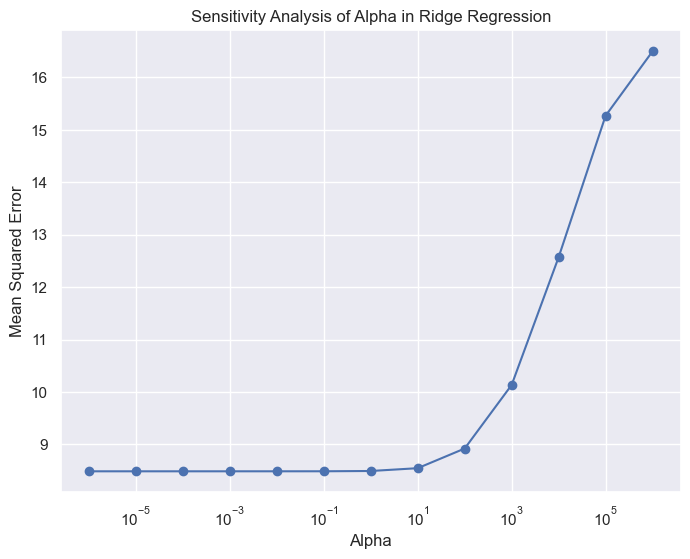
\includegraphics[width=0.5\linewidth]{sensitivity.png}
    \caption{Sensitivity Analysis of Alpha in Ridge Regression}
    \label{fig:enter-label}
\end{figure}



\section{Strengths and Weaknesses}
\subsection{Strengths}
\begin{itemize}
    \item RidgeCV automatically selects the optimal value of α using cross-validation. This reduces the need for manual tuning and helps avoid the risk of overfitting or underfitting that might occur when selecting $\alpha$ by hand.
    \item XGBoost efficiently handles missing values during training, reducing preprocessing needs and retaining valuable information. This feature is ideal for large, complex datasets, such as Olympic predictions, ensuring robustness despite incomplete data.


\end{itemize}



\subsection{Weaknesses}
\begin{itemize}
    \item While RidgeCV helps with regularization, it does not perform feature selection. The model will retain all features, but it will shrink the coefficients of less important features towards zero. In situations where feature selection is critical, other techniques like Lasso (which uses L1 regularization) may be more appropriate.
\end{itemize}






% 参考文献,此处以 MLA 引用格式为例
\begin{thebibliography}{99}
\bibitem{1}
Nielsen.
\newblock Nielsen’s Gracenote Expects USA, China, Great Britain, France and Australia to Lead 2024 Paris Olympic Games Medal Table.
\newblock \url{https://www.nielsen.com/news-center/2024/virtual-medal-table-forecast/}.

\bibitem{2}
Moolchandani, Jhankar, et al.
\newblock "Predictive Analytics in Sports: Using Machine Learning to Forecast Outcomes and Medal Tally Trends at the 2024 Summer Olympics."
\newblock \textit{2024 4th International Conference on Technological Advancements in Computational Sciences (ICTACS)}.
\newblock 2024.
\newblock \url{https://ieeexplore.ieee.org/document/10840553}.

\bibitem{3}
Sergeyev, Yaroslav D.
\newblock \textquotedblleft The Olympic Medals Ranks, lexicographic ordering and numerical infinities.\textquotedblright
\newblock \textit{arXiv preprint arXiv:1509.04313}, 11 Sep. 2015.
\newblock Available: \url{https://arxiv.org/abs/1509.04313}.

\bibitem{4}
Tianqi Chen and Carlos Guestrin.
\textit{XGBoost: A Scalable Tree Boosting System}.
In \textit{Proceedings of the 22nd ACM SIGKDD International Conference on Knowledge Discovery and Data Mining}, 2016.

\bibitem{5}
Zhang, P., Jia, Y., \& Shang, Y. (2022). Research and application of XGBoost in imbalanced data. \textit{International Journal of Distributed Sensor Networks}, 18(6). \textit{doi:10.1177/15501329221106935}

\bibitem{6}
Li, J., Liu, H., Yang, Z., \& Han, L. (2021). A Credit Risk Model with Small Sample Data Based on G-XGBoost. \textit{Applied Artificial Intelligence}, 35(15), 1550--1566. \url{https://doi.org/10.1080/08839514.2021.1987707}

\bibitem{7}
Shi, R., Xu, X., Li, J., \& Li, Y. (2021). Prediction and analysis of train arrival delay based on XGBoost and Bayesian optimization. \textit{Applied Soft Computing}, 109, 107538. \url{https://doi.org/10.1016/j.asoc.2021.107538}

\bibitem{8}
Wu, J., Chen, X. Y., Zhang, H., Xiong, L. D., Lei, H., \& Deng, S. H. (2019). Hyperparameter optimization for machine learning models based on Bayesian optimization. \textit{Journal of Electronic Science and Technology}, 17(1), 26-40.

\bibitem{9}
Saito, T., and M. Rehmsmeier.
\textit{The precision-recall plot is more informative than the ROC plot when evaluating binary classifiers on imbalanced datasets}.
\textit{PLoS One} 10.3 (2015): e0118432.
\textit{doi: 10.1371/journal.pone.0118432}.

\bibitem{10}
Liang, Xiaodan.
\textit{Analysis of the Development Trend of China's Competitive Track and Field Events from the Results of the 18th Asian Games Track and Field Competition}.
\textit{Journal Name} 10.2 (2019): 123-145.

\bibitem{11}
McKnight, Patrick E., and Julius Najab.
\textit{Mann‐Whitney U Test}.
\textit{The Corsini encyclopedia of psychology} 1-1 (2010): 1-1.
\textit{doi: 10.1002/9780470479216.corpsy0524}.

\bibitem{12}
Mardia, K. V.
\textit{Small Sample Power of a Non-Parametric Test for the Bivariate Two-Sample Location Problem in the Normal Case}.
\textit{Journal of the Royal Statistical Society Series B: Statistical Methodology} 80.1 (2018): 1-24.
\textit{doi: 10.1111/jrss.b.2018.80.issue-1}.

\bibitem{13}
Csurilla, Gergely, and Imre Fertő.
\textit{The less obvious effect of hosting the Olympics on sporting performance}.
\textit{Scientific Reports} 13 (2023): 819.
\textit{doi: 10.1038/s41598-022-27259-8}.




\end{thebibliography}


% 以下为附录内容
% 如您的论文中不需要附录,请自行删除
\begin{subappendices}  % 附录环境


\section{Appendix A: Program Codes}
Here are the program codes we used in our research.

% 代码环境示例三则
% 如您的论文不需要展示代码,请删除
% 更多用法,请参考 listings 宏包文档

% Python 代码示例
\begin{lstlisting}[language=Python]
# Sliding Windows
medals_expand = medals.copy()
def add_lag_features(df, lag=4):
    # Group by NOC 
    for i in range(1, lag + 1):
        # Create features for the previous i Olympic Games: number of medals, totals, etc.
        medals_expand[f'Gold_Lag{i}'] = medals_expand.groupby('NOC')['Real_Gold'].shift(i)
        medals_expand[f'Silver_Lag{i}'] = medals_expand.groupby('NOC')['Real_Silver'].shift(i)
        medals_expand[f'Bronze_Lag{i}'] = medals_expand.groupby('NOC')['Real_Bronze'].shift(i)
        medals_expand[f'Athletes_Lag{i}'] = medals_expand.groupby('NOC')['Athletes'].shift(i)
        medals_expand[f'Females_Lag{i}'] = medals_expand.groupby('NOC')['Females'].shift(i)
        medals_expand[f'Sports_Lag{i}'] = medals_expand.groupby('NOC')['Sports'].shift(i)
        medals_expand[f'Events_Lag{i}'] = medals_expand.groupby('NOC')['Events'].shift(i)
        medals_expand[f'Athletes per Event_Lag{i}'] = medals_expand.groupby('NOC')['Athletes per Event'].shift(i)
    return(df)
medals_expand = add_lag_features(medals_expand, lag=9)
\end{lstlisting}
\begin{lstlisting}[language=Python]
def bootstrap_resample(X_predict, y_train):
  # Bootstrap parameters
  n_iterations = 2000
  n_size = len(X_Scaled_train)
  # Store Prediction Outcomes
  predictions = np.zeros((n_iterations, len(X_predict)))
  # Bootstrap Resample
  for i in range(n_iterations):
      # Randomn Sampling
      X_resample, y_resample = resample(X_Scaled_train, y_train, n_samples=n_size)
      # Train
      model.fit(X_resample, y_resample)
      # Predict
      predictions[i, :] = model.predict(X_predict)
  # Calculate Prediction Intervel
  lower_bound = np.percentile(predictions, 2.5, axis=0)
  upper_bound = np.percentile(predictions, 97.5, axis=0)
  return lower_bound, upper_bound
\end{lstlisting}

\end{subappendices}  % 附录内容结束

\end{document}  % 结束
